A vtp fájlok megjelenítéséhez a legegyszerűbb megoldás 
a prt megjelenítő alkalmazás továbbfejlesztése lett volna.
Ezt végül elvetettem a következő hátrányok miatt:
\begin{itemize}
\item Az AntTweakBar felület külső megjelenése 
nem hasonlít egy modern alkalmazáséra.
\item A prt megjelenítő alkalmazásnál problémát okozott 
a betöltendő fájlok kiválasztása, 
amit végül nem is sikerült rendesen megcsinálni. 
Erre sajnos se a GLFW, se az AntTweakBar 
nem tartalmaz beépített megoldást.
\item A prt megjelenítő alkalmazásnál sajnos 
le kellett mondani a kamera egérrel 
történő középpont körüli forgathatóságáról, 
mivel ez akadályozta volna az interakciót 
az AntTweakBar felülettel, 
ami szintén az OpenGL ablakba rajzolta magát.
\item 
A prt megjelenítő alkalmazás osztályait 
úgy terveztem meg, 
hogy a részecskék generálása és a generált részecskék mozgatása könnyen 
és gyorsan történhessen. 
A vtp fájloknál viszont nem kell semmit se mozgatni, 
ahogy nem kell egyszerre több fájlt se betölteni 
a megjelenítéshez (a prt fájloknál a részecskék sebességét 
a rendszer a pozíciók különbsége alapján számolja ki, 
amihez mindig két egymás utáni fájlt is be kell tölteni).
\end{itemize}
A felsorolt hátrányok miatt végül egy teljesen különálló 
vtp megjelenítő alkalmazás készült. 
Az alkalmazás legfontosabb jellemzői:
\begin{itemize}
\item A vtp fájlok gyors betöltése.
\item Modern kezelőfelület a megjelenítés vezérléséhez és a fájlok betöltéséhez.
\item Megjelenítés egy külön OpenGL ablakban, 
a felhasználói felülettől függetlenül.
\item Platformfüggetlenség. 
Az alkalmazás működik Windows 10 és Linux környezetekben, 
továbbá lefordul GCC -vel, MinGW -vel és 
a Microsoft hivatalos C++ fordítójával is.
\end{itemize}

\section{A fejlesztéskor használt könyvtárak}

\begin{description}[font=\normalfont\itshape\space]
\setlength{\parindent}{2ex}
\item [Megjelenítés] \hfill \\
A fentiek alapján OpenGL -en kívül még lehetett volna a Vulkan API -t is választani, 
azonban ennek kicsi az elterjedtsége és támogatottsága, 
így a döntés végül az OpenGL -re esett.
\item [kezelőfelület] \hfill \\
Az alkalmazás a Qt -t használja. Lehetett volna a gtk -t is választani, 
ami szintén elterjedt, a könyvtár mérete jóval kisebb 
és csak grafikus felhasználói felületet tartalmaz. 
Hátránya, hogy bonyolultabbak a függvényhívások és 
a Qt -hez képest szegényesebb a dokumentáció. 
További előnye a Qt -nak, hogy a csomagban olyan eszközök is vannak, 
mint a qmake, vagy a Qt Creator, 
amik jelentősen megkönnyíthetik a Qt -ban történő fejlesztést.
\item [fájlok betöltése] \hfill \\
A vtp fájlok betöltéséhez a legegyszerűbb megoldás természetesen 
a VTK könyvtár használata lett volna. 
A könyvtárral a gond a mérete és komplexitása volt. 
Emiatt egyrészt sok helyet foglalt volna, másrészt használata, 
valamint annak megtanulása fölöslegesen sok időt vett volna igénybe, 
mivel az alkalmazásnak csak pár meghatározott típusú 
egyszerű vtp fájlt kell megnyitnia. 
A fejlesztéskor az is fontos cél volt, 
hogy az alkalmazás lehetőség szerint kicsi maradjon 
és minél kevesebb külső könyvtártól függjön. \\
Szerencsére a Qt a grafikus felhasználói felületen kívül 
rengeteg más szolgáltatást is tartalmaz. 
Ilyen például QXmlStreamReader osztály, 
ami lehetővé teszi az xml fájlok beolvasását 
és feldolgozását külső könyvtárak nélkül. 
Ez a célra tökéletesen megfelelt, 
mivel a betöltendő vtp fájlok is xml formátumúak.
\end{description}

\section{A Qt szoftverfejlesztési csomag}

A vtp fájlok betöltésére és megjelenítésére írt alkalmazás 
a prt megjelenítővel szemben az OpenGL -t leszámítva C++ függvénykönyvtárból 
egyedül a Qt -t használja. 
A Qt -ra eredetileg a benne szereplő grafikus felület miatt esett a választás, 
azonban a később kiderült, 
hogy ennél jóval többet tud 
és gyakorlatilag az összes fejlesztéskor felmerülő külső könyvtárat 
képes kiváltani saját megoldásokkal.

\subsection{A Qt története}

A Qt fejlesztését Eirik Chambe-Eng és Haavard Nord kezdte el 1990 nyarán. 
Ők ekkoriban egy C++ alapú adatbázis -kezelő alkalmazáson dolgoztak, 
amiben ultrahang képeket kellett megjeleníteni. 
Az alkalmazás grafikus felhasználói felületének működnie kellett Unix -on, 
Macintosh- on és Windows -on is. 
A két fejlesztő egyik akkori megoldással sem volt megelégedve, ezért úgy döntöttek, 
felépítenek az
alapoktól egy cross platform objektum -orientált grafikus felhasználói felületet. 
Miután 1993 -ra az alapvető osztályok elkészültek, 
az eredmény láttán a fejlesztők alapítottak egy céget és úgy döntöttek, 
hogy megcsinálják „a világ 
legjobb C++ GUI keretrendszerét” \cite{qthistory}. 
A cég eredeti neve Quasar technologies volt, amit később átneveztek Trolltech -re. 
Ekkoriban találták ki a Qt elnevezést is az Xt, 
azaz X toolkit nevű függvénykönyvtár alapján. 
A Q betűt egyébként a kinézete miatt választották, 
külön jelentése nincs.

Az első nagyobb cégek, amik fejlesztéshez a Qt -t használták, 
a norvég Metis és az Európai Űrügynökség voltak. 
Az igazi áttörést a Qt számára azonban a KDE jelentette 1997 -ben, 
amikor a projekthez ezt a szoftverfejlesztési csomagot választották. 
A KDE egy grafikus felhasználói felület Linux operációs rendszerekhez, 
ami 1999 -re a legelterjedtebb felületek közé tartozott, 
ezzel biztosítva a Qt népszerűségét is.

A 2000 -es években aztán sok más céghez hasonlóan Trolltech is a mobil 
és beágyazott rendszerek felé fordult.
Ennek is köszönhető, hogy végül a Nokia felvásorlta.
Mindezek ellenére nem fejeződött be 
a Qt asztali operációs rendszerekre szánt könyvtárainak és 
szolgáltatásainak fejlesztése.

Manapság a Qt asztali könyvtárait olyan projektek használják, 
mint a KDE plasma 5, vagy az LxQt, 
amik a Linux legelterjedtebb felhasználói felületei közé tartoznak.

\subsection{Qt Widgets}

A Qt programcsomagban jelenleg két modul is található 
grafikus felhasználói felület készítéséhez:  
a Quick és a Widgets. 
A Quick újabb és jóval modernebb. 
Hátránya, hogy mobilra és tabletre optimalizálták,
így egy asztali operációs rendszeren nem néz ki jól. 
A Widgets fejlesztésekor ezzel szemben a cél kifejezetten 
az asztali környezetekbe való illeszkedés volt. 

A Widgets különlegessége, hogy Macintosh -on és Windows -on nem 
az operációs rendszer részét képező UI elemeket használja, 
hanem helyette sajátokat implementál \cite{qtdocumentation}. 
Ennek következtében lehetőség van például 
Windows környezetben is Mac stílusú alkalmazás készítésére.

A vtp fájlok betöltéséhez és megjelenítéshez írt 
alkalmazás a Widgets modult használja.

\vspace{2mm}

\noindent{\itshape\bfseries A Qt Widgets fontosabb tulajdonságai:}

\vspace{2mm}

\begin{itemize}
\item 
A fő ablakot is beleértve minden, 
a felületen látható elem a QWidget osztályból származik le.
\item 
A Widgetekkel kapcsolatos események kezelése 
a később bemutatásra kerülő signal/slot rendszerrel történik. 
\item
A QWidget nem absztrakt osztály, 
tehát önmagában is használható például más felületelemek tárolására.
\item
A felhasználói felület tervezhető hagyományos módon
a C++ kódban
és tervezhető XML nyelven egy .ui fájlban is. 
A vtp megjelenítő alkalmazás az utóbbi módszert használja.
\item 
A Qt az alap felületelemeken kívül lehetőséget 
biztosít azokból leszármazott osztályok használatára is. 
Ez igaz mind a hagyományos tervezésre, mind a .ui fájlokra.
\item
Bár a Widget -ek kinézete alapértelmezetten 
a használt operációs rendszertől függ, 
a Qt tartalmaz egy Style Sheets szolgáltatást, 
amivel ez felülírható és testreszabható. 
A Qt megoldását 
a HTML Cascading Style Sheets inspirálta \cite{qtdocumentation}, 
ami érezhető is a használat folyamán.
\end{itemize}

\vspace{2mm}

\noindent{\itshape\bfseries
A vtp megjelenítő -ben használt fontosabb Qt felületelemek:}

\vspace{2mm}

\begin{sloppypar}
\begin{description}[font=\normalfont\itshape\space]
\item [QLabel, QSlider, QSpinBox, QCheckBox, QComboBox:] 
A funkciójuk megegyezik a natív Windows -os megfelelőjükkel. 
Sajnos a QSlider -ből a QSpinBox -szal ellentétben nincs lebegőpontos változat, 
ami projektben sok osztály implementációját is befolyásolta.
\item [QPushButton:] 
A Windows gomb elemének felel meg. 
A projektben legtöbbször a leszármazott {\ttfamily ColorButton} szerepel, 
ami megnyomáskor feldob egy színkiválasztó ablakot, 
majd tárolja a kiválasztott színt.
\item [QToolButton:] 
Az eszköztáron az action -ök ilyen gombok formájában jelennek meg. 
A vtp megjelenítő alkalmazásban a eszköztárakon kívül 
a gomb szerepel a fájlmegnyitó ablakon is, 
ahol az előre és vissza gombokat valósítja meg.
\item [QLineEdit:] 
A Windows -ban található szövegdoboz Qt -s megfelelője.
\item [Spacer:] 
Funkciója csak annyi, hogy két felületelem között kihagy valamekkora helyet.
\item [QMenuBar, QMenu:] 
A felhasználói felület tetején a menüsort a {\ttfamily QMenuBar} osztály valósítja meg, 
amin belül az egyes elemek a {\ttfamily QMenu} -k.
\item [QToolBar:] A Windows -ban jellemző eszköztár elemnek felel meg. 
Tartalmaz egy {\ttfamily toogleViewAction} függvényt, 
ami visszaad egy olyan menühivatkozást a felső menüsorhoz, 
amivel az eszköztár megjeleníthető és eltüntethető.
\item [QAction:] 
Az osztály egy általános interfészt biztosít olyan utasítások végrehajtására, 
mint például a megnyitás, 
vagy mentés. 
Az action -ok felhasználói felülethez nem kötött objektumok, 
amiknek szükség esetén a felhasználói felületen is 
lehet reprezentációja például egy gomb formájában, 
ugyanakkor be lehet állítani gyorsbillentyűt is. 
Egy action -höz a grafikus felületen tetszőleges számú gomb tartozhat, 
azonban egy alkalmazásban tipikusan két gombot szoktak elhelyezni, 
amik közül az egyik a menüsor valamelyik elemébe, 
a másik egy eszköztárra szokott kerülni. 
\item [QDockWidget:] A {\ttfamily QDockWidget} lényegében egy panel, 
ami lehet külön ablakban, 
vagy lehet dock -olva a főablakba. 
A főablakban a {\ttfamily QDockWidget} -eknek 4 hely van fenntartva. 
Ezek az ablak alsó és felső, valamint a bal és jobb széle. 
A {\ttfamily QDockWidget} -en alapértelmezetten található a jobb felső sarokban 
egy close gomb is, amivel a panel eltüntethető. 
A {\ttfamily QDockWidget} -hez is van {\ttfamily toogleViewAction} függvény, 
így könnyen készíthető olyan Action, 
ami képes bezárni, vagy megjeleníteni a panelt.
\item [QHBoxLayout, QVBoxLayout:] 
Elrendezések, amik a bennük lévő teret vízszintesen, 
illetve függőlegesen osztják fel. 
Működésük nagyjából megegyezik a Windows megfelelő osztályával. 
A vtp megjelenítő alkalmazásban a fájlkiválasztó ablak használja.
\item [QFormLayout:] 
Egy Qt specifikus elrendezés, 
amit kifejezetten változók beállítására terveztek. 
Az elrendezés két oszlopot tartalmaz. 
Az egyikben {\ttfamily QLabel} -ek, 
a másikban „editor” elem -ek találhatók 
(Pl.: {\ttfamily QLineEdit} vagy {\ttfamily QSpinBox}). 
Mivel a sorokba lehetőség van olyan elemet is tenni, 
ami az egész sort kitölti (erre a {\ttfamily QSlider} -ek miatt volt szükség), 
a {\ttfamily QFormLayout} alkalmasnak bizonyult arra, 
hogy elrendezze a dock -olható panelek tartalmát.
\item [QMainWindow:] 
Ez az osztály biztosítja az ablakot az alkalmazás számára. 
Ahogy a \ref{fig:x mainWindowsLayout} ábrán is látszik, 
középen egy tetszőleges típusú QWidget helyezkedik el, 
amit körbevesz a dock -olható paneleknek, 
majd az eszköztáraknak kijelölt terület. 
Ezenkívül megtalálható rajta legfelül a szokásos menüsor, 
míg alul a status bar is.
\par
\begin{figure}[!htb]
\centering
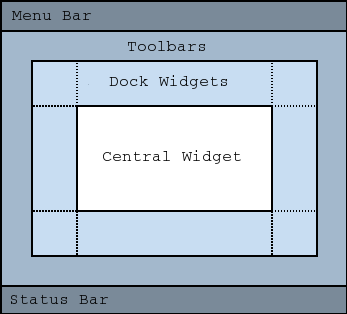
\includegraphics[scale=0.7]{mainwindowlayout}
\caption{QMainWindow elrendezése \cite{mainwindowlayout}}
\label{fig:x mainWindowsLayout}
\end{figure}
\par
\item [QOpenGLWidget:] 
Egy különleges widget, 
amire OpenGL segítségével lehet rajzolni. 
Az OpenGL függvények az osztály tagfüggvényeiként vannak implementálva. 
Ennek egyik előnye, 
hogy lehetővé teszi, 
hogy egymástól teljesen függetlenül
lehessen rajzolni egyszerre több 
QOpenGLWidget -re is.
A rajzolás történhet a hivatalos OpenGL függvényeivel
és a Qt saját fejlesztésű OpenGL wrapper API -jával is,
ami a C stílusú OpenGL hívásokat 
QOpenGL kezdetű objektumorientált osztályokba csomagolja. 
A Qt függvényeinek használata egyszerűségükön 
és jól olvashatóságukon kívül azért is előnyös, 
mert az API elfedi az OpenGL és az OpenGL ES közötti különbségeket, 
ezzel biztosítva a kód kompatibilitását a különböző eszközökkel. 
A vtp megjelenítő alkalmazás fejlesztésekor 
a sima OpenGL függvények voltak preferálva,
mivel a fejlesztés második szakaszában a cél különböző könyvtáraktól, 
így a Qt -tól való függés minimalizálása volt.
\item [QListWidget:] 
A Windows -ban található listanézetnek felel meg. 
Az vtp megjelenítő alkalmazásban 
a fájlkiválasztó ablak használja a meghajtók és 
a fontosabb mappák megjelenítésére.
\item [QTreeView:] 
A Qt -ban a {\ttfamily QTreeWidget} osztály felel meg 
a Windows treeview osztályának. 
A {\ttfamily QTreeView} funkciókra megegyezik a {\ttfamily QTreeWidget} -tel, 
csak azzal ellentétben tartalmának meghatározása 
a Qt Model/View technikájával történik. 
Az osztály a vtp megjelenítő alkalmazás szempontjából
a fájlkiválasztó ablak miatt volt fontos,
ahol egy {\ttfamily QTreeView} -n jelennek meg a fájlok.
\end{description}
\end{sloppypar}

\subsection{Signal -ok és slot -ok}

A signal/slot mechanizmus a Qt különleges szolgáltatása, 
aminek célja a kommunikáció megkönnyítése a felhasználói felület elemei
és egyéb objektumok között. 
A rendszer a Qt sajátossága, 
tehát a többi C++ függvénykönyvtárra nem jellemző.
Egy hagyományos függvénykönyvtárban a kommunikáció 
callback függvények segítségével történik. 
Ez a módszer a következőképpen foglalható össze:

A rendszerben minden UI elemhez előre definiálva vannak különböző események. 
Ilyen esemény lehet például egy gomb esetén az, 
ha rákattintanak az egérrel.

Az alkalmazásban vannak olyan függvények, 
amik átvesznek egy értesítést arról, 
hogy egy adott UI elemmel egy adott esemény bekövetkezett
és eldöntik, hogy a program milyen választ adjon. 
Ezeket eseménykezelő eljárásnak, vagy callback függvénynek hívják.

Az UI elemek amikor bekövetkezik rajtuk egy esemény, 
mindig meghívják az összes 
(a legtöbb függvénykönyvtárban csak egy darab callback függvény megadására van lehetőség) 
annak kezelésére írt callback függvényt. 
Ehhez a callback függvényeket persze regisztrálni kell.
A callback függvények regisztrálása 
valamilyen formában (Pl.: C\# esetén delegate -ok) 
mindig az eseménykezelő eljárásokra mutató pointer(-ek) átadásával történik.

A Qt erre kínál egy másfajta megközelítést a signal és slot alapú kommunikációval, 
ami a következő elvek alapján működik:

\begin{itemize}
\item A UI komponenseknek lehetőségük van signal -okat definiálni, 
amik a kódban definíció nélküli függvénydeklarációként jelennek meg.
\item A UI komponenseknek lehetőségük 
van signal -okat kibocsájtani 
(a dokumentációban „emit” \cite{qtmodelview}). 
A hagyományos C++ függvénykönyvtárban jellemző események 
a Qt -s megfelelői signal -okkal vannak definiálva.
\item A UI komponenseknek lehetőségük van slot -okat definiálni. 
A slot -ok void visszatérésű függvények, 
amik célja egy adott típusú esemény kezelése.
\item A különböző UI komponensek signal -jai és slot -jai összeköthetőek egymással. 
Egy signal kapcsolódhat több slothoz, 
egy slot kapcsolódhat több signalhoz.

Signal -jai és slot -jai csak megpéldányosított objektumoknak lehetnek, 
osztályoknak nem. 
Egy signal egy slot -tal akkor is összeköthető, 
ha a signal -t és a slot -ot tartalmazó objektum osztálya megegyezik. 
Egy signal összeköthető olyan slot -al is, 
ami ugyanabban az objektumpéldányban található. 
Ezenkívül lehetőség van egy signal -t hozzákötni egy másik signal -hoz is.
\item Amikor egy UI komponens kibocsájt egy signal -t, 
egymás után minden hozzákötött slot meghívódik 
minden tartalmazó objektumra külön. 
Ha egy signalhoz egy másik signal van kötve, kibocsájtáskor annyi történik, 
hogy a másik signal is kibocsájtásra kerül.
\item Signal -okat és Slot -okat minden olyan osztály definiálhat, 
ami a {\ttfamily QObject} osztályból származik, 
tehát jelzéseket nem UI komponensek is tudnak küldeni.
\end{itemize}

A fenti szabályokból látható, 
hogy a Qt signal/slot rendszere egy hagyományos 
C++ függvénykönyvtárban nem lenne megvalósítható, 
mivel például signal elem nincs a C++ -ban. 
Ennek megoldására tervezték a Qt Meta-Object rendszerét. 
Ennek lényege, hogy a Qt -hez tartozik egy Meta-Object Compiler, 
ami a signal -okat vagy slot -okat tartalmazó osztályokban 
egy {\ttfamily Q\_OBJECT} macro segítségével metaadatokat helyez el 
mielőtt a kód a tényleges C++ fordítóhoz kerülne. 
A módszer hátránya természetesen az, 
hogy bár a kód fordítófüggetlen marad, 
a Qt eszközei sajnos megkerülhetetlenek lesznek a fordításhoz.

A továbbiakban egy példán keresztül bemutatásra kerül, 
hogyan történik a signal -ok és slot -ok definiálása, 
valamint összekapcsolása egy Qt projektben.

Az első osztályban egy függvény és egy signal található. 
A függvény feladata annyi, hogy ha meghívják, 
az osztály kibocsájt egy signal -t a paraméterként átadott üzenettel. 
A kódból jól látható a signal -ok definiálásának 
és kibocsájtásának szintaktikája is. 
A definiálás lényegében egy függvénydeklarációval történik, 
amit egy {\ttfamily „signal:”} label előz meg. 
A kibocsájtást az {\ttfamily emit} kulcsszóval lehet előidézni. 
A kódban az is látható, 
hogy az osztály elején ott van a kötelező {\ttfamily Q\_OBJECT} macro, 
aminek helyére a Meta-Object Compiler a signal/slot rendszer 
működéséhez szükséges kódot teszi:
\begin{lstlisting}[style=customcpp]
class EventEmitter : public QObject
{
    Q_OBJECT
public:
    void emitEvent(QString message);
signals:
    void eventSignal(QString message);
};
\end{lstlisting}
Az {\ttfamily emitEvent} függvény definíciója:
\begin{lstlisting}[style=customcpp]
void EventEmitter::emitEvent(QString message)
{
    emit eventSignal(message);
}
\end{lstlisting}
\begin{sloppypar}
\setlength{\parindent}{0ex}
A második osztályban egy slot található, 
ami az átvett üzenetet kiírja a kimenetre. 
Ahogy a kódban is látszik, a slot -ok megkülönböztetése 
a többi függvénytől a {\ttfamily „slot:”} label segítségével történik:
\end{sloppypar}
\begin{lstlisting}[style=customcpp]
class EventReceiver : public QObject
{
    Q_OBJECT
public slots:
    void eventSlot(QString message);
};
\end{lstlisting}
Az eventSlot definíciója:
\begin{lstlisting}[style=customcpp]
void EventReceiver::eventSlot(QString message)
{
    qDebug() << "Message received: " << message;
}
\end{lstlisting}
\begin{sloppypar}
A main függvény az osztályok példányosítása után 
összekapcsolja az {\ttfamily EventEmitter} signal -ját 
az {\ttfamily EventReceiver} -ben található slot -tal, 
majd meghívja az {\ttfamily EventEmitter} signal -t kibocsájtó függvényét. 
A kódban van egy {\ttfamily QObject::connect} függvény is. 
Ezzel történik a signal -ok slot -okhoz való kötése:
\end{sloppypar}
\begin{lstlisting}[style=customcpp]
int main()
{
    EventEmitter emitter;
    EventReceiver receiver;
    QObject::connect(&emitter, &EventEmitter::eventSignal, 
                     &receiver, &EventReceiver::eventSlot);
    emitter.emitEvent("sample message");
    return 0;
}
\end{lstlisting}

A Qt signal -slot rendszerének több előnye is van. 
Egyrészt így a signal -t és a slot -ot tartalmazó osztályok 
architekturális értelemben nem függenek egymástól, 
másrészt a rendszer programozási szempontból 
egyszerű és magától értetődő \cite{qtsignalslot}. 
A signal/slot rendszer modern változatának további előnye, 
hogy fordítási időben biztosítja az osztályok és 
callback függvények típusának helyességét (Ez a korábbi Qt verziókra még nem volt igaz). 

\subsection{A Qt matematikai szolgáltatásai}

A vtp megjelenítő alkalmazás a kamera mátrixainak kiszámítására, 
valamint a pozíciók és színek tárolására a prt fájloknál is alkalmazott 
GLM helyett a Qt beépített osztályait használja. 
Ezen belül a {\ttfamily QVector3D} és a {\ttfamily QMatrix4x4}  
osztályokra volt szükség, 
amiket főleg a kamera használ.

A Qt vektor és mátrix osztályai bár nagyon jók abból a szempontból, 
hogy az alkalmazás a Qt -n kívül tényleg semmilyen külső osztálytól nem függ, 
használatuknak vannak hátrányai is. 
Ezek közül a legfontosabb, hogy a GLM vektor osztályával ellentétben 
a Qt dokumentációja nem garantálja, 
hogy a {\ttfamily QVector3D} adatstruktúrája csak 
három darab lebegőpontos értéket tartalmazzon,
ahogy azt se, hogy ezek a helyes sorrendben legyenek. 
Emiatt az OpenGL -nek nem lehet közvetlenül a {\ttfamily QVector3D} -ket átadni, 
hanem először át kell másolni a vektorok adatait egy float tömbbe. 
Bár kevésbé jelent problémát, 
de néha zavaró tud lenni, hogy a Qt osztályai a GLM -el ellentétben 
nem immutable objektumok, 
tehát például a mátrixok esetén a transzformációk 
a mátrix belső állapotán változtatnak ahelyett, 
hogy egy új mátrix -szal térnének vissza. 
A GLM -el szemben további gyengeség a függvények viszonylag alacsony száma. 
Erre egyik példa a vektorok tengely körül történő forgatása, 
ami a Qt -ban csak a forgatási mátrix felépítésével, 
majd ezzel való szorzással lehetséges, 
míg a GLM -ben a művelet egy egyszerű függvényhívással megoldható.

\subsection{QXmlStreamReader}

Az osztály egyszerű és gyors megoldást biztosít 
xml formátumú szövegek beolvasására és feldolgozására. 
A betöltés stream alapon történik, 
tehát az osztály a szöveget folytonosan olvassa be 
és nem néz a szövegben előre, vagy hátra. 
Ennek előnye, hogy a beolvasás gyors és a memóriában egyszerre 
csak a fájl egy minimális része található.

A {\ttfamily QXmlStreamReader} működésének alapja, 
hogy az xml szöveget „token” -nek nevezett egységekre bontja és ezeket egyenként, 
egymás után olvassa be. 
Tokenekből több -féle is lehet. A következő tipikus xml elem esetén:
\begin{lstlisting}[style=customxml]
<Data name="PI" type="Float32">3.1415926</Data>
\end{lstlisting}
Például a {\ttfamily QXmlStreamReader} három különböző típusú token -t fog beolvasni:
\begin{description}[font=\normalfont\small\ttfamily\space]
\item [<Data name="PI" type="Float32">:] 
Ez egy {\ttfamily StartElement} típusú token.
\item [3.1415926:] 
Ez egy {\ttfamily Characters}.
\item [</Data>:] 
Ez pedig egy {\ttfamily EndElement}.
\end{description}
Az xml szövegek feldolgozásakor ez a három token a legfontosabb 
(A projekthez csak ezek kellettek), de sok egyéb típus is van.

Az osztály használatát szemléltetendő, 
a következőkben bemutatásra kerül egy egyszerű xml fájl, 
valamint egy ennek betöltésére írt példakód. 
Bár a vtp megjelenítő alkalmazásban ennél bonyolultabb kód található, 
annak működése lényegileg nem különbözik ettől.

A betöltendő példa xml fájl egy darab gyökér elemet tartalmaz, 
amin belül található két szöveg és egy lebegőpontos szám. 
A fájl szerkezete egyébként nagyon hasonlít a megjelenítendő vtp fájlokra:
\begin{lstlisting}[style=customxml]
<?xml version="1.0"?>
<DataFile>
    <Data name="text 1" type="text">The first text</Data>
    <Data name="PI" type="Float32">3.1415926</Data>
    <Data name="text 2" type="text">The second text</Data>      
</DataFile>
\end{lstlisting}
Példakód a fájl beolvasására:
\begin{lstlisting}[style=customcpp]
int main()
{
    QFile inputFile("D:/cpp_projects/QtXmlExampleProject/example.xml");
    QXmlStreamReader reader(&inputFile);
    if (!inputFile.open(QIODevice::ReadOnly))
    {
            qDebug() << "Failed to open file";
            return 1;
    }
    bool wasOpeningTextData = false;
    while (!reader.atEnd())
    {
        QXmlStreamReader::TokenType type = reader.readNext();
        if(type == QXmlStreamReader::StartElement)
        {
            qDebug() << "Opening tag: " << reader.name();
            if(reader.name() == "Data" 
                    && reader.attributes().value("type") == "text")
            {
                wasOpeningTextData = true;
            }
        }
        else if(wasOpeningTextData == true 
                && type == QXmlStreamReader::Characters)
        {
            qDebug() << reader.text();
            wasOpeningTextData = false;
        }
        else if(type == QXmlStreamReader::EndElement)
        {
            qDebug() << "Closing tag: " << reader.name();
        }
    }
    return 0;
}
\end{lstlisting}
A példakódban egy main függvény látható, 
aminek két feladata van. 
Egyrészt kiírja a Qt debug kimenetére, 
ha nyitó, vagy záró tag -hez ért, másrészt kiírja a megtalált adatot, 
ha az szöveg típusú volt.

\begin{sloppypar}
A függvény a fájl megnyitásával, 
majd a megnyitott fájl alapján a 
{\ttfamily QXmlStreamReader} inicializálásával kezdődik. 
Ezután az xml fájl beolvasása következik egy while cikluson keresztül. 
A cikluson belül egy egyszerű állapotgép van. 
Ha a betöltött token típusa egy olyan nyitó tag ({\ttfamily StartElement}) 
amiben a {\ttfamily „Data”} név szerepel, 
valamint a {\ttfamily type} attribútum értéke {\ttfamily „text”}, 
a ciklus egy szöveges adathoz érkezett, 
ami azt jelenti, 
hogy a következő token maga a kiírandó szöveg lesz. 
Ez lejegyzésre kerül a {\ttfamily wasOpeningTextData} változóba. 
Ennek megfelelően ha a ciklus egy {\ttfamily „Characters”} tokenhez érkezett, 
a {\ttfamily wasOpeningTextData} változó alapján már el tudja dönteni, 
hogy a token szöveg -e, vagy lebegőpontos szám. 
Szöveg esetén a kiírás után ilyenkor visszaállításra kerül 
a {\ttfamily wasOpeningTextData} változó is. 
Amennyiben a ciklus egy befejező taghez érkezett ({\ttfamily EndElement}), 
kiírja, hogy closing tag, 
valamint kiírja a tag -ben szereplő szót.
\end{sloppypar}

A példából látszik, 
hogy {\ttfamily QXmlStreamReader} használata jóval egyszerűbb 
sok, szintén xml feldolgozáshoz írt könyvtárnál. 
További előnye, 
hogy a fájlból egyszerre csak egy token -t tart a memóriában, 
így lehetőség van nagyon nagy, 
sok adatot vagy elemet tartalmazó fájlok hatékony feldolgozására is. 
A {\ttfamily QXmlStreamReader} igazi ereje azonban abban rejlik, 
hogy lehetőség van vele olyan xml beolvasókat létrehozni, 
amik képesek a feladat egy részét átadni egy másik függvénynek. 
Például ha lenne az xml fáljban egy olyan {\ttfamily „Data”} elem is, 
ami gyerekelemeket tartalmaz, 
az ilyen elemek feldolgozását akár át lehetne adni egy másik függvénynek, 
hiszen a betöltés abban is ugyan úgy, 
szekvenciálisan mehetne tovább.

\subsection{A Qt egyéb hasznos osztályai}

A Qt több egy egyszerű grafikus felhasználói felületnél. 
A tervezők célja egy olyan fejlesztői környezet létrehozása volt, 
amivel bármilyen asztali alkalmazással kapcsolatos 
probléma megoldható külső könyvtárak használata nélkül is. 
A továbbiakban pár olyan osztály kerül bemutatásra, 
amik fontosak voltak a vtp megjelenítő alkalmazás fejlesztésekor.
\begin{description}[font=\normalfont\itshape\space]
\item [QVector:] 
Az osztály célja az {\ttfamily std::vector} típus leváltása. 
A Qt beépített container osztályainak
az legfontosabb előnye az STL -lel szemben, 
hogy míg az stl osztályoknál 
elvileg minden fordítókörnyezet szabadon dönthet az implementálás módjáról, 
a Qt -s osztályoknak csak egy darab, 
jól dokumentált implementációja létezik. 
A vtp megjelenítő alkalmazásnál persze inkább 
a {\ttfamily QVector} azon előnye volt a fontos, 
hogy jobban együttműködik a Qt többi osztályával.
\item [QString:] 
Az osztály az STL {\ttfamily std::string} típusának leváltására készült. 
Legfontosabb előnye, 
hogy támogatja a különböző karakterkódolások használatát, 
valamint a szöveg átalakítását az egyik karakterkódolásból a másikba. 
A karakterek tárolása ennek megfelelően nem egy 8 bites, 
hanem utf -16 formátumban történik. 
\item [QDir:] 
Az osztály feladata a fájlkezelés segítése. 
A projekt szempontjából a legfontosabb funkciója, 
hogy le lehet vele kérdezni egy listát a mappában található fájlokról.
\item [QFile:] 
Az osztály feladata, 
hogy egy modern, a magasabb szintű nyelvekre 
jellemző felületet biztosítson fájlok kezeléséhez. 
Legfontosabb szolgáltatása természetesen a fájlok beolvasása és kiírása, 
de lehetőség van fájlok meglétének ellenőrzésére, 
másolására és törlésére is. 
Beolvasáshoz és kiíráshoz a {\ttfamily QFile} -t 
általában stream objektumokkal szokás használni, 
amik a fájlból beolvasott adatot a megfelelő célformátumúvá alakítják. 
A {\ttfamily QTextStream} például a szövegek, 
míg a {\ttfamily QDataStream} binárisan tárolt változók beolvasására alkalmas. 
A projekt szempontjából a {\ttfamily QXmlStreamReader} osztály volt fontos, 
mivel ez tölti be vtp fájlokat. 
\item [QFileInfo:]
Az osztály képes egy adott fájllal kapcsolatban 
olyan információk lekérdezésére, 
mint például a fájl mérete vagy módosítási dátuma. 
A projektben a saját fájlkiválasztó ablak használja.
\end{description}

\subsection{A Qt előnyei és hátrányai 
a prt megjelenítő alkalmazásnál használt 
függvénykönyvtárakhoz képest}

\begin{description}[font=\normalfont\itshape\space]
\item [Előnyök:] \hfill
\begin{enumerate}
\item
A felhasználói felület jóval professzionálisabb kinézetű 
és hasonlít a modern Windows -os asztali alkalmazások felületére.
\item
A Qt -ban az AntTweakBar -ral ellentétben a kezelőfelület 
külön van választva az OpenGL ablaktól, 
így lehetőség volt a kamera egérrel történő forgatásának implementálására is.
\item
Bár Számozott fájlokból álló fájlkötegek kiválasztására 
alkalmas párbeszédablak sajnos nincs a Qt -ban, 
a Qt Widgets modul lehetőséget biztosított egy ilyen megírására.
\item
Mivel a vtp fájlok xml formátumúak, 
szükség volt egy olyan függvénykönyvtárra, 
ami képes xml fájlok betöltésére és egyszerű feldolgozására. 
Szerencsére a Qt tartalmaz ilyet is.
\item
A Qt -hez tartozó qmake build eszköz jóval könnyebben használható 
a többi hasonló megoldásnál, 
miközben a CMake -hez hasonlóan biztosítja 
a projekt platformtól és fordítótól való függetlenségét. 
A qmake további előnye az alkalmazás szempontjából 
az erőforrásfájlok (például vertex és fragment shader) 
egyszerű hozzáadása a projekthez.
\end{enumerate}
\item [Hátrányok:] \hfill
\begin{enumerate}
\item
Bár a Qt projektek platform és fordítófüggetlenek, 
csak a Qt -hez tartozó qmake build eszközzel fordíthatóak. 
Ennek következtében nincs lehetőség a prt megjelenítőnél 
látott módon hozzáadni külső függőségeket, 
mivel a CMake -el ellentétben a qmake használata 
annyira nincs elterjedve 
(Bár nem Qt -s projekt is build -elhető vele). 
\item
Bár a Qt resource rendszere biztosítja az erőforrások egyszerű 
és praktikus kezelését, 
az erőforrások így csak a Qt osztályaival tölthetőek be, 
ami további függést jelent.
\item
Az OpenGL alapú rajzolás alapból nem valósítható meg olyan osztályokban, 
amik kívül esnek a Qt ökoszisztémáján. 
Ennek következménye, hogy a kirajzolást végző kód 
nem hasznosítható újra más projektekben.
\item
Hasonló problémát eredményez a signal/slot rendszer használata, 
ami bár leegyszerűsíti az osztályok közötti kommunikációt, 
megakadályozza az osztályok nem Qt alapú projektekben történő újrahasznosítását.
\end{enumerate}
\end{description}

\section{Qt Model/View}

Egy alkalmazásban gyakran van szükség listák, 
táblák és fa struktúrák megjelenítésére. 
A megjelenítendő adatok és a felületelem közötti kapcsolathoz
a Qt két megközelítést is támogat.

Az egyik, hogy a felületelem
a megjelenő tartalmat belső változókban tárolja,
amiket kívülről kell frissíteni.
A legtöbb C++ GUI könyvtárban egyébként ez a jellemző.
A megközelítés előnye, hogy a megjelenítendő adatok megadása egyszerű, 
mivel azokat elég csak átadni egy függvénynek (Pl.: {\ttfamily addRow}). 
Ezen kívül a felületelemmel kapcsolatos kódok rövidek és magától értetődőek, 
ami növeli az olvashatóságot és a programozás sebességét.

A megközelítés hátránya, 
hogy az adatokat feleslegesen több helyen is tárolni kell, 
valamint hogy a felület és az adatok közötti szinkronizáció nehézkes lehet. 
Ezek különösen akkor jöhetnek elő, 
ha ugyanazt a tartalmat egyszerre több helyen is meg kell jeleníteni.

A Qt másik lehetséges megközelítése 
a Model/View programozás \cite{qtmodelview}. 
Ilyenkor a Widget -ek nem tárolják a rajtuk megjelenő adatokat, 
hanem külső objektumokból töltik be azokat 
egy előre meghatározott interfészen keresztül. 
A Model/View programozás hátránya, 
hogy kevésbé intuitív, 
így első látásra sokkal bonyolultabbnak tűnhet. 
Előnye viszont, hogy így az adatokat csak egyszer kell tárolni, 
miközben akármennyi Widget -en megjelenhetnek. 
Ezen kívül a szinkronizációval sem kell foglalkozni, 
hiszen az adatok megváltozása egyből változást eredményez 
az azt megjelenítő összes Widget -en is.

A vtp megjelenítő alkalmazás a Qt Model/View programing módszerét 
a fájlkiválasztó ablakban található {\ttfamily QTreeView} -nél használta. 
A QTreeView funkciója az aktuális mappa tartalmának megjelenítése, 
valamint ezen van lehetőség a megjelenítendő fájlok tényleges kiválasztására is.

\subsection{Model-View-Controller}

A Model/View programing -nál alkalmazott architektúrához 
az ötletet Model-View-Controller tervezési minta 
eredeti Smalltalk -os változata adta \cite{qtmodelview}. 
Ennek lényege, hogy a felhasználói felület elemeinek működtetésében 
három fajta objektum vesz részt \cite{mvchistory}: \newline
A Model objektumok a felületen megjelenítendő adatot tárolják.\newline
A View objektumok valamely Model objektum egy vizuális reprezentációját jelentik. 
Egy Model -hez egyébként több View is tartozhat. \newline
A Controller objektumokban található 
a felhasználói interakcióval kapcsolatos események kezelése, 
valamint szükség esetén itt történik a Model objektumok frissítése.
\begin{figure}[!htb]
\centering
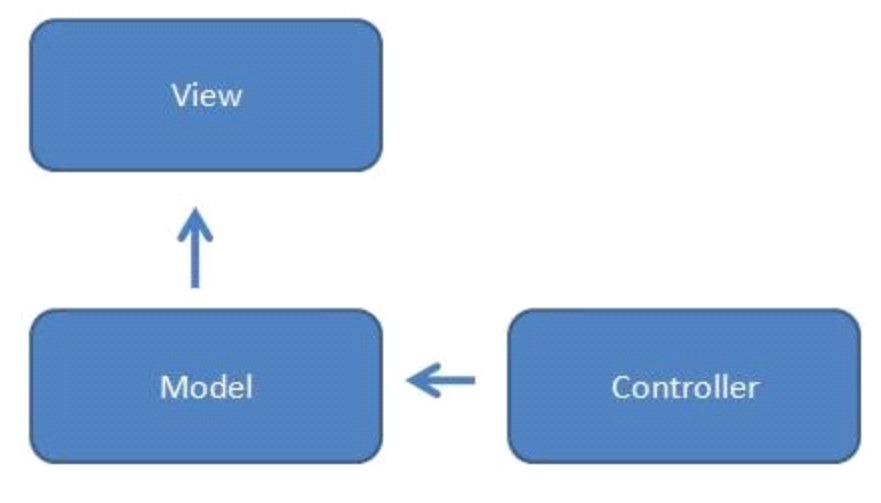
\includegraphics[scale=0.8]{mvcOriginal}
\caption{Az eredeti MVC minta \cite{mvcoriginal}}
\label{fig:x mvc}
\end{figure}

Ahogy a \ref{fig:x mvc} ábrán is látható, 
az eredeti Smalltalk -os változatban a View -t a Model értesíti a változásokról. 
Ez különbözik több mai elterjedt MVC értelmezéstől. 
Jó példa erre az ASP.NET MVC, 
ahol a Model és a View között a kapcsolatot a Controller teremti meg.

\subsection{A Qt Model/View programming architektúrája}

A Qt Model/View programming alapötlete, 
hogy a View részhez hozzáveszi a Controller funkciót is. 
Így egy olyan architektúra jön létre, ami továbbra is szétválasztja 
az adatok tárolásának és vizuális reprezentációjának logikáját egymástól, 
ezzel biztosítva a MVC tervezési mintára jellemző 
rugalmasságot és újrafelhasználhatóságot, 
miközben az eredeti MVC -hez képest 
a programozás egyszerűbb marad \cite{qtmodelview}.

A Qt Model/View programming architektúrája természetesen 
az MVC -hez hasonlóan továbbra is lehetővé teszi, 
hogy ugyanazokat az adatokat a tárolás logikájának megváltoztatása 
nélkül lehessen egyszerre megjeleníteni akár több,
egymástól különböző felületen is. 
\begin{figure}[!htb]
\centering
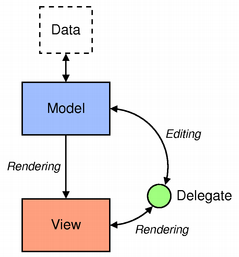
\includegraphics[scale=0.7]{modelview-overview}
\caption{A Qt Model/View architektúra \cite{mvprogramming}}
\label{fig:x QtModelView}
\end{figure}

Ahogy a \ref{fig:x QtModelView} ábrán is látszik, 
a Model/View architektúra osztályai három csoportba sorolhatóak:
a Model, a View és a Delegate.

A Model osztályok feladata, 
hogy kommunikáljanak az adatok forrásával
és egy interfészt biztosítsanak azok elérésére. 
Az adatok jöhetnek kívülről (például adatbázis szerver), 
vagy tárolódhatnak akár a Model osztályok belső változójaként is. 

A View osztályok felelnek meg 
a felhasználói felületen látható Widget -eknek, 
amik az adatok megjelenítését végzik. 

A Delegate osztályok feladata az egyes adatok kirajzolása a View -ra, 
valamint az adatok View -n történő módosításakor 
a módosítás érvényre juttatása a Model osztályokban.
Delegate -ek felüldefiniálásával biztosítható például, 	
hogy hőmérsékletszám helyett a felületen egy hőmérőcsíkot tartalmazó ábra jelenjen meg, 	
valamint azt is így lehet elérni, hogy
egy táblázat tartalmának szerkesztésekor ne szövegdoboz,       	
hanem spinBox jelenjen meg a táblázat adott cellájában.
A vtp megjelenítő alkalmazás fejlesztésekor szerencsére megfeleltek 
az alapértelmezett Delegate osztályok is, 
mivel a fájlkiválasztó felület adatait nem kellett sem szerkeszteni, 
sem különleges módon megjeleníteni. 

A Model, View és Delegate komponensek 
a Qt -ban absztrakt osztályként vannak megvalósítva, 
ezzel biztosítva a kommunikációhoz szükséges interfészek meglétét. 
Saját osztályok készítéséhez mindig ezekből kell leszármazni.

A Model, View és Delegate komponensek közötti kommunikáció természetesen 
a Qt signal/slot rendszerével történik. 
A Model signal -ok segítségével értesíti 
a View -t a mögötte lévő adatok megváltozásáról, 
a View signal -okat bocsájt ki a felhasználói interakcióról, 
a Delegate pedig az adatok felületen történő módosítása 
közben signal -ok segítségével értesíti a model -t és a view -t 
a megváltozott értékekről. 

\subsection{A Model osztályok közös interfésze}

Ahogy fentebb már említésre került, 
a Model osztályok feladata, 
hogy egy egységes interfészt biztosítsanak 
a View és Delegate osztályoknak az adatok elérésére. 
Ezt a Qt fejlesztői úgy valósították meg,
hogy az adatok tényleges tárolási módjától függetlenül 
a Model osztályok az adatokat egy fa struktúra formájában reprezentálják, 
ahol egy csomópontban egymás mellett több elem is tárolódik. 

Bár a Qt dokumentációjából a megvalósítás mögötti motiváció nem derül ki, 
valószínűleg ezzel az lehetett a cél, 
hogy egy olyan Model interfészt biztosítsanak, 
ami ugyanúgy használható 
a {\ttfamily QListView}, a {\ttfamily QTableView} 
és {\ttfamily QTreeView} osztályokkal is, annak ellenére, 
hogy a {\ttfamily QTreeView} struktúrája kicsit más.

A Következőkben bemutatásra kerül az osztályok által reprezentált fa struktúra 
egy gyakorlati példán keresztül is.
\begin{figure}[!htb]
\centering
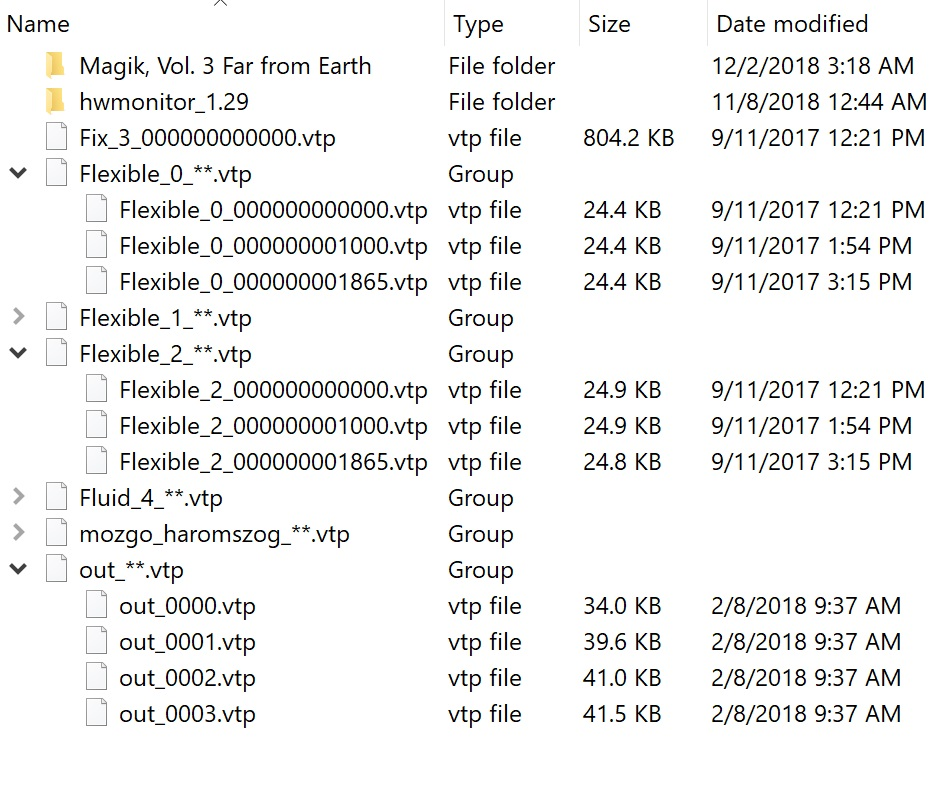
\includegraphics[scale=1.1]{treeviewexample}
\caption{példa QTreeView -re}
\label{fig:x treeviewexample}
\end{figure}
\newline
A \ref{fig:x treeviewexample} ábrán egy {\ttfamily QTreeView} látható, 
amiben fájlok, fájlcsoportok és mappák információi vannak. 
A Model ezt a következőképpen reprezentálja:
\begin{itemize}
\item
Minden sorral és oszloppal azonosítható információ 
egy elemmek (a dokumentációban item) felel meg a Model -ben,
tehát egy elem reprezentálja a „file folder” felirat, 
illetve a „24.4 KB” mögötti adatot is.
\item
A lenyitatlan sorokban minden elem szülője a gyökérelem (rootitem).
\item
A lenyitott sorokban további sorok láthatóak. 
A bennük lévő elemek szülője mindig a lenyitott sor első eleme, 
tehát a példában az az elem, ami a fájlnevet szolgáltatja.
\end{itemize}

A Model objektumok közös interfészét a Qt úgy biztosítja, 
hogy minden Model osztálynak a 
{\ttfamily QAbstractItemModel} leszármazottjának kell lennie. 
A Qt -ban ezen kívül vannak további kényelmi Model osztályok is, 
amik implementálják a {\ttfamily QAbstractItemModel} egyes függvényeit. 
Ilyen például {\ttfamily QAbstractListModel}, 
vagy a {\ttfamily QAbstractTableModel}, 
amik a {\ttfamily QListView}, 
illetve {\ttfamily QTableView} osztályok használatát könnyítik meg. 

\subsection{Model indexek}

A View -ben, vagy a View -t használó osztályokban gyakran szükség van 
egy elem adatainak lekérdezésére (például az elemen történő kattintáskor, 
vagy kirajzoláskor). 
A Qt, hogy szétválassza az adatok tényleges reprezentációját az elérés módjától, 
az adatok elérésére bevezette az indexeket. 
Az index alapvetően úgy viselkedik, 
mintha egy pointer lenne a Model egy elemére. 
Fontos különbség viszont, 
hogy az indexek csak ideiglenes referenciaként funkcionálnak, 
tehát tárolni például semmiképp sem szabad őket. 
A következőkben bemutatásra kerül az indexek három legfontosabb használati esete:
\begin{description}[font=\normalfont\itshape\space]
\item [Index lekérdezése egy adott elemhez: ] \hfill \\
A {\ttfamily QAbstractItemModel} {\ttfamily index} függvényével történik. 
A függvény első két paramétere a sor és oszlop, 
a harmadik pedig a szülőelem indexe. 
Ha a függvény hívásakor szülőelemként a gyökérelem átadására van szükség, 
ez a {\ttfamily QModelIndex()} konstruktor hívásával tehető meg. 
A konstruktorral készített index ugyanis mindig a gyökérelemre mutat.
\item [Felhasználói adat lekérdezése az index -től: ] \hfill \\
Az indexek lehetőséget biztosítanak egy pointer tárolására, 
ami tetszőleges típusú objektumra mutathat. 
Ennek lekérdezése az index {\ttfamily internalPointer} függvényével történik. 
Ha egy View eseménykezelő eljárásában (például egy kattintás kezelésekor) 
szükség van valamilyen adatra az adott elemmel kapcsolatban, 
a Qt példaprojektjei alapján ezt célszerű használni, 
illetve a Model -t is célszerű úgy implementálni, 
hogy az {\ttfamily internalPointer} a szükséges objektumra mutasson.
\item [Megjelenítendő adatok lekérdezése index alapján:] \hfill \\
Erre a Model {\ttfamily data} függvénye használható, 
ami egy tetszőleges Qt -n belül definiált objektummal tér vissza. 
A {\ttfamily data} függvény alapvetően azt a célt szolgálja, 
hogy a Qt beépített osztályai számára biztosítsa
az elem megjelenítéséhez szükséges adatokat. 
Emiatt mindenképp implementálni kell, 
bár a függvény eseménykezelő eljárásban történő használata 
egy bonyolultabb Model esetén nem célszerű. 
A {\ttfamily data} függvénynek egy adott elemmel kapcsolatban több, 
különböző típusú adat visszaadására is képesnek kell lennie. 
Ezt a Qt úgy oldja meg, 
hogy a {\ttfamily data} függvény a lekérdezendő elem indexén kívül 
átvesz egy {\ttfamily role} enum -ot is, 
ami a visszaadandó objektum típusát és tartalmát határozza meg. 
A fájlok böngészéséhez készített TreeView esetén például 
az elő oszlop elemeinél {\ttfamily DisplayRole} esetén a fájl nevével, 
{\ttfamily DecorationRole} -nál pedig a fájl
ikonjával kellett visszatérni. 
Ha valamely {\ttfamily role} esetén nincs szükség visszatérési értékre 
(Például a táblázatban a név mellé nem kell ikon), 
a data függvénynek egy {\ttfamily QVariant} típusú objektummal kell visszatérnie. 
\end{description}

\section{A vtp megjelenítő alkalmazás specifikációja}

A vtp fájlok betöltéséhez a prt megjelenítő alkalmazáshoz képest 
egy „professzionálisabb” felületű alkalmazás készült, 
aminek kezelőfelülete hasonlít a Windows -ban megszokotthoz.

\subsection{Fájlok betöltése}

A fájlok betöltése és megjelenítése két módon történhet. 
Egyrészt be lehet tölteni egyszerre egy darab fájlt, 
másrészt ha egy mappában több azonos nevű számozott vtp fájl található, 
lehetőség van ezek egyszerre történő betöltésére is. 
Utóbbi esetben a program a betöltött fájlokat sorba rendezi 
a nevükben szereplő szám szerint, 
majd az egyes fájlokat egy animáció frame -jeinek tekintve 
egymás után jeleníti meg. 
A lejátszás vezérléséhez a felhasználói felületen természetesen megtalálhatóak 
a média lejátszókból is ismert gombok.
Ezenkívül van egy opció az aktuális frame számának közvetlen megadására, 
valamint a maximális másodpercenkénti képkockaszám meghatározására is.

A betöltendő fájlok kiválasztásához a prt megjelenítővel ellentétben 
az alkalmazás tartalmaz egy fejlett párbeszédablakot. 
Ezen lehetőség van egy Windows explorerhez hasonló felületen böngészni 
a számítógépen található vtp fájlokat. 
A párbeszédablak különlegessége, 
hogy az azonos nevű számozott fájlokat lenyitható csoportokba rendezi.

A párbeszédablakon a felhasználó egyszerre csak egy darab fájlt 
vagy fájlcsoportot tud kiválasztani a betöltéshez. 
Ezzel az alkalmazás biztosítja, 
hogy a felhasználónak ne legyen lehetősége több olyan fájl megnyitására, 
amik nem ugyanahhoz az animációhoz tartoznak.

\subsection{OpenGL ablak és kamera}

A vtp fájlok megjelenítése egy OpenGL ablakban történik. 
Az alkalmazás a fájlok betöltésekor kiszámítja a megjelenítési tér középpontját, 
ami az egyes frame -ek részecskepozícióinak összesített átlaga. 
A kamera mindig erre a pontra néz, 
azonban a többi paramétere állítható. 
Az OpenGL ablakon a bal vagy jobb egérgomb nyomva tartásával 
lehetőség van a kamera középpont körül történő forgatására. 
Az egér görgőjével a kamera közelíthető, 
illetve távolítható a középponthoz képest. 
Az alkalmazásban található egy kamera panel, 
amin az említett beállításokon kívül megadható a látószög is.

\subsection{A vtp fájlok kirajzolása}

A fájlok tartalmának megjelenítésére a program tartalmaz 
egy részecske és egy háromszögrajzoló módot.

Részecskerajzoló módban a program 
a fájlokban található pozíciók helyére pontokat rajzol. 
Ez azoknál a fájloknál kapcsolódik be automatikusan, 
amikben nincsenek indexek.
A fejlesztés folyamán ugyanis az volt a tapasztalat, 
hogy az ilyen fájloknál általában a pozíciók 
egymás utáni háromszögpontoknak tekintése furcsa eredményt adna. 

Háromszögrajzoló módban a program 
a fájlokból betöltött pozíciókat háromszögpontoknak tekinti, 
amiket a betöltött indexek szerinti sorrendben, 
vagy index nélküli fájlok esetén, egymás utáni sorrendben rajzol ki. 
Ha a fájlban vannak indexek is, 
alapértelmezetten ez a mód kapcsolódik be.

Sajnos egyik megjelenítendő fájl sem tartalmaz színeket és normálvektorokat. 
Emiatt háromszögrajzoló módban ezeknek a meghatározása is a programra hárul. 
Az alkalmazásba végül külön normálvektorszámító algoritmus nem került, 
így a kirajzolt háromszögek egyenes felületűek maradtak.
\newline
Az alkalmazás a pontok színének meghatározására három lehetőséget kínál fel:
\begin{description}[font=\normalfont\itshape\space]
\item [solid:]
Ebben a módban a pontok egyszerűen 
a felhasználói felületen beállított színt veszik fel. 
A lehetőséget a program minden fájl esetén felajánlja.
\item [velocity:]
Ha a betöltött fájl tartalmaz a pontokhoz {\ttfamily „velocity”} információt, 
lehetőség van színezni a sebességvektorok abszolút értéke szerint is. 
Ez egy felhasználói felületen megadható start és end szín alapján történik. 
A program megkeresi az animációhoz tartozó összes frame -ben együttvéve 
a legkisebb és legnagyobb sebességértéket. 
Ezután egy pont színét úgy határozza meg, 
hogy a megtalált minimális sebesség a start, 
a maximális pedig az end színt fogja jelenteni. 
A többi pont egy két szín közötti interpolált értéket kap.
\item [vertex area, projected vertex area és vertex mass:]
Erre a három módra akkor van lehetőség, 
ha a betöltött fájl tartalmaz a pontokhoz egy {\ttfamily „area”} nevű információt is. 
Bár az {\ttfamily „area”} a {\ttfamily „velocity”} -hez 
hasonlóan a fájlokban három elemű vektorként van definiálva, 
a három számot az egyes pontok esetén külön kell értelmezni. 
Az x koordináta felel meg a {\ttfamily „vertex area”}, 
az y a {\ttfamily „projected vertex area”}, 
a z pedig a {\ttfamily „vertex mass”} értéknek. 
A színezés ezekben a módokban is hasonlóan történik a velocity módhoz, 
csak a vektorok abszolút értékei helyett a megfelelő koordináták számítanak.
\end{description}

\subsection{Megvilágítás}

A vtp fájlok kirajzolásakor az alkalmazás egy pontfényforrást használ. 
A fényforrásnak állítható a pozíciója, ereje és színe. 
Ezenkívül lehet állítani a visszaverődő fény intenzitását, 
valamint a test felületének a simaságát is.

A program egy további fontos funkciója, 
hogy a fényforrást a fájlok betöltésekor mindig 
a megjelenítési tér közepéhez viszi. 

\subsection{A vtp megjelenítő alkalmazás felhasználói felülete}

\begin{figure}[!htb]
\centering
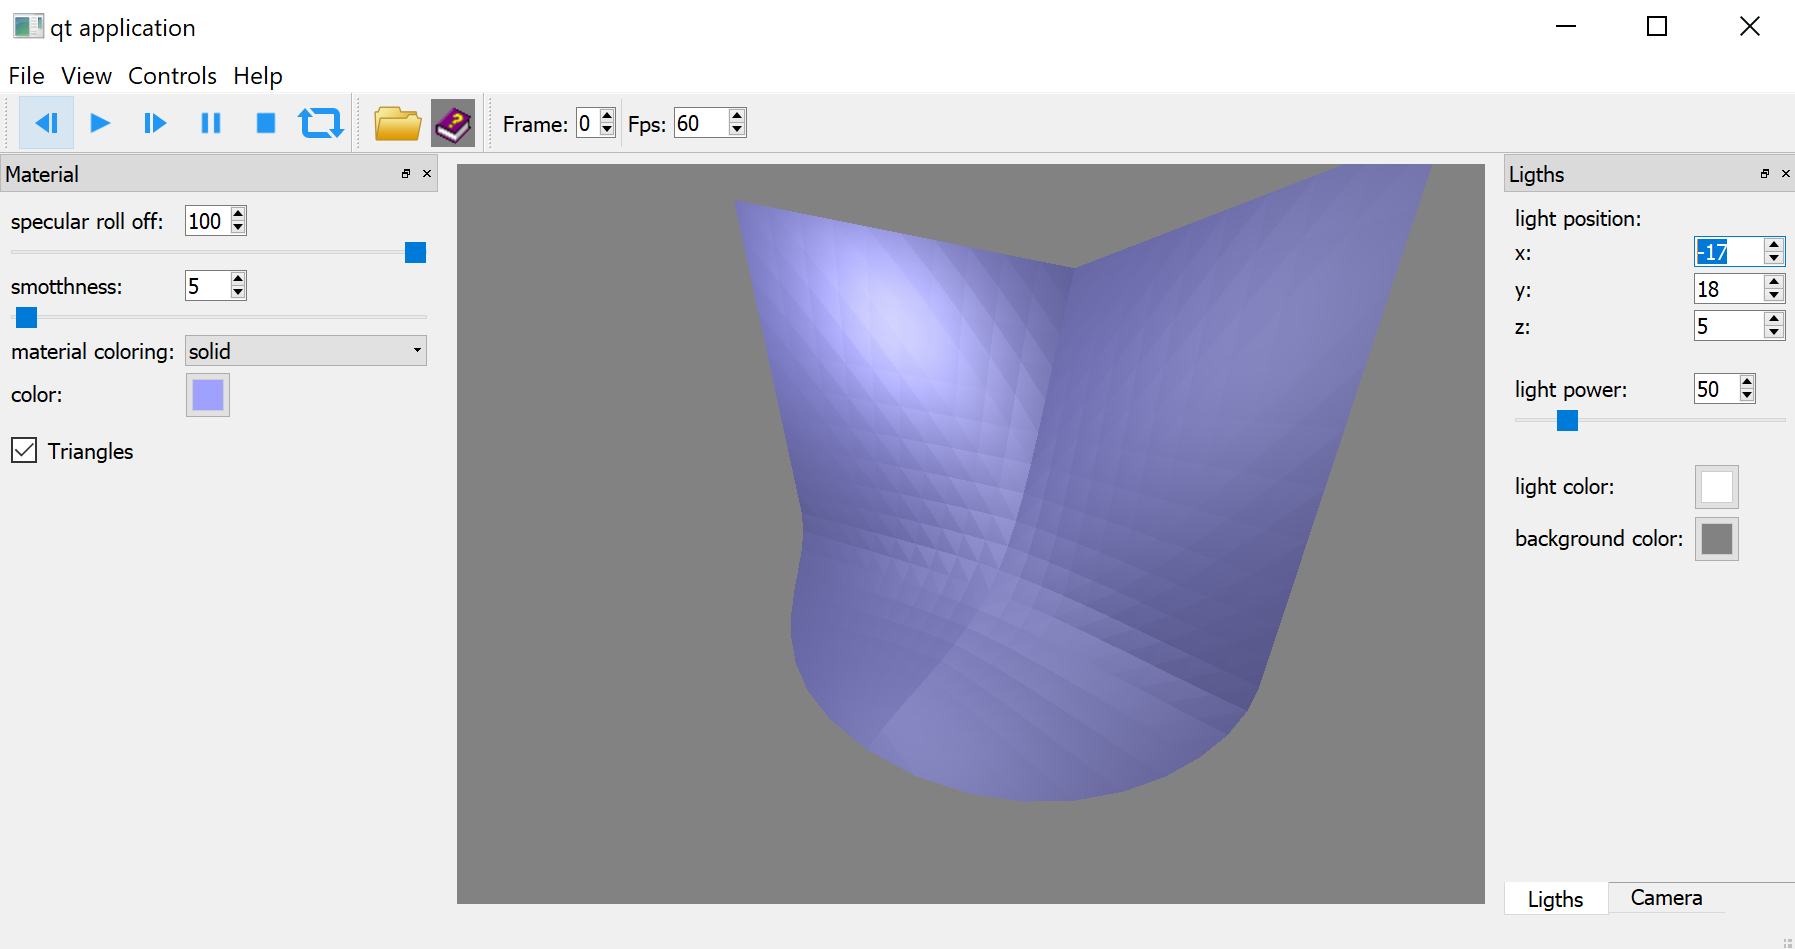
\includegraphics[scale=0.64]{szakdoga_gui}
\caption{A vtp megjelenítő alkalmazás felhasználói felülete}
\label{fig:x szakdogaGui}
\end{figure}
Ahogy a \ref{fig:x szakdogaGui} ábrán is látszik, 
az alkalmazás közepén egy OpenGL ablak található. 
Ebben történik a vtp fájlok megjelenítése. 
A felületen van még három dock -olható panel, 
három eszköztár és a felső részen egy menüsor is.
\begin{description}[font=\normalfont\itshape\bfseries\space]
\item [Material panel:] \hfill \\
Itt azok a kirajzolással kapcsolatos beállítások találhatóak, 
amik csak a kirajzolandó test anyagától függenek, 
az egyes fényforrások tulajdonságaitól nem.
\begin{description}[font=\normalfont\itshape\space]
\item [specular roll off:]
Egy 0 és 100 közötti szám, 
amit a program 0 és 1 közötti lebegőpontos értékre képez. 
A felületről visszaverődő fény erősségét lehet vele állítani.
\item [smoothness:]
Minél magasabb az érték, 
annál simábbnak látszódik a felület, 
ha a spekuláris szín be van kapcsolva.
\item [material coloring:]
Itt lehet választani a színezési módok között.
\item [color, start color, end color:]
A színezési módtól függően itt lehet állítani a színeket.
\item [triangles:] 
Ezzel állítható, hogy a program háromszögeket vagy pontokat rajzoljon.
\end{description}
\item [Lights panel:]
\begin{description}[font=\normalfont\itshape\space]
\item []
\item [light position:]
A fényforrás pozíciója.
\item [light power:]
A fényforrás ereje.
\item [light color:]
A fényforrás színe.
\item [background color:]
A háttér színe.
\end{description}
\item [Camera panel:]
\begin{description}[font=\normalfont\itshape\space]
\item []
\item [horizontal angle:]
A kamera elfordulási szöge az y tengely körül.
\item [vertical angle:]
A kamera függőleges szöge. 
A program az x tengely körüli forgatást követően 
ezzel a szöggel forgatja el a kamerát 
a kamerához képest jobbra mutató vektor körül.
\item [distance:]
A kamera távolsága a középpontól.
\item [field of view:]
A kamera látószöge.
\end{description}
\item [File load eszköztár:]
\begin{description}[font=\normalfont\itshape\space]
\item []
\item [Open File:]
A gomb hatására előjön egy párbeszédablak, 
amin ki lehet választani a betöltendő vtp fájlokat.
\item [About:]
Egy rövid leírást tartalmaz a programról.
\end{description}
\item [Frames eszköztár:]
\begin{description}[font=\normalfont\itshape\space]
\item []
\item [Frame:]
Itt állítható, hogy a program hanyadik frame -et jelenítse meg.
\item [Fps:]
Lejátszáskor a maximális fps szám.
\end{description}
\item [Media controls eszköztár:] \hfill \\
Az eszköztáron hat darab gomb található, 
amikkel a vtp fájlok egymás utáni kirajzolását lehet állítani 
egy médialejátszóhoz hasonló módon. 
Ezek a Play, Stop, Pause, előző és következő frame, 
valamint Replay gombok.
\item [A menüsor elemei:]
\begin{description}[font=\normalfont\itshape\space]
\item []
\item [File:]
Ebben egy kilépés, valamint a File Load eszköztáron is 
elhelyezett Open File gomb található.
\item [View:]
Itt lehet megjeleníteni és elrejteni az 
alkalmazás eszköztárait és dock -olható paneljeit.
\item [Controls:]
Itt is megtalálhatóak a Media Controls eszköztár elemei.
\item [Help:]
Ide egyelőre az eszköztáron is megjelenő About gomb került. 
\end{description}
\end{description}

\section{A vtp megjelenítő alkalmazás megvalósítása}

Az alkalmazás tervezésekor a prt megjelenítőhöz hasonlóan 
itt is fontos szempont volt, 
hogy a fájlok betöltését végző rész különváljon 
az OpenGL specifikus kirajzolással kapcsolatos részektől 
és a user input kezelésétől. 
Sajnos az utóbbi kettőt nem lehetett szétválasztani. 
Ennek oka, hogy az OpenGL függvényeit 
az OpenGL ablakot megvalósító osztályon belül kell meghívni, 
viszont a Qt signal/slot rendszere miatt itt találhatóak 
az eseménykezelő eljárások is. 

Az OpenGL specifikus részek leválasztására egyébként 
az alkalmazás már tartalmaz egy megoldást ({\ttfamily OpenGLInterface} osztály), 
azonban ezen keresztül csak 
a shaderek betöltéséhez szükséges OpenGL függvényeket lehet meghívni, 
a többit egyelőre nem.

A következőkben ismertetésre kerül az alkalmazás architektúrája, 
valamint a fontosabb osztályok feladatai:

\begin{figure}[!htb]
\centering
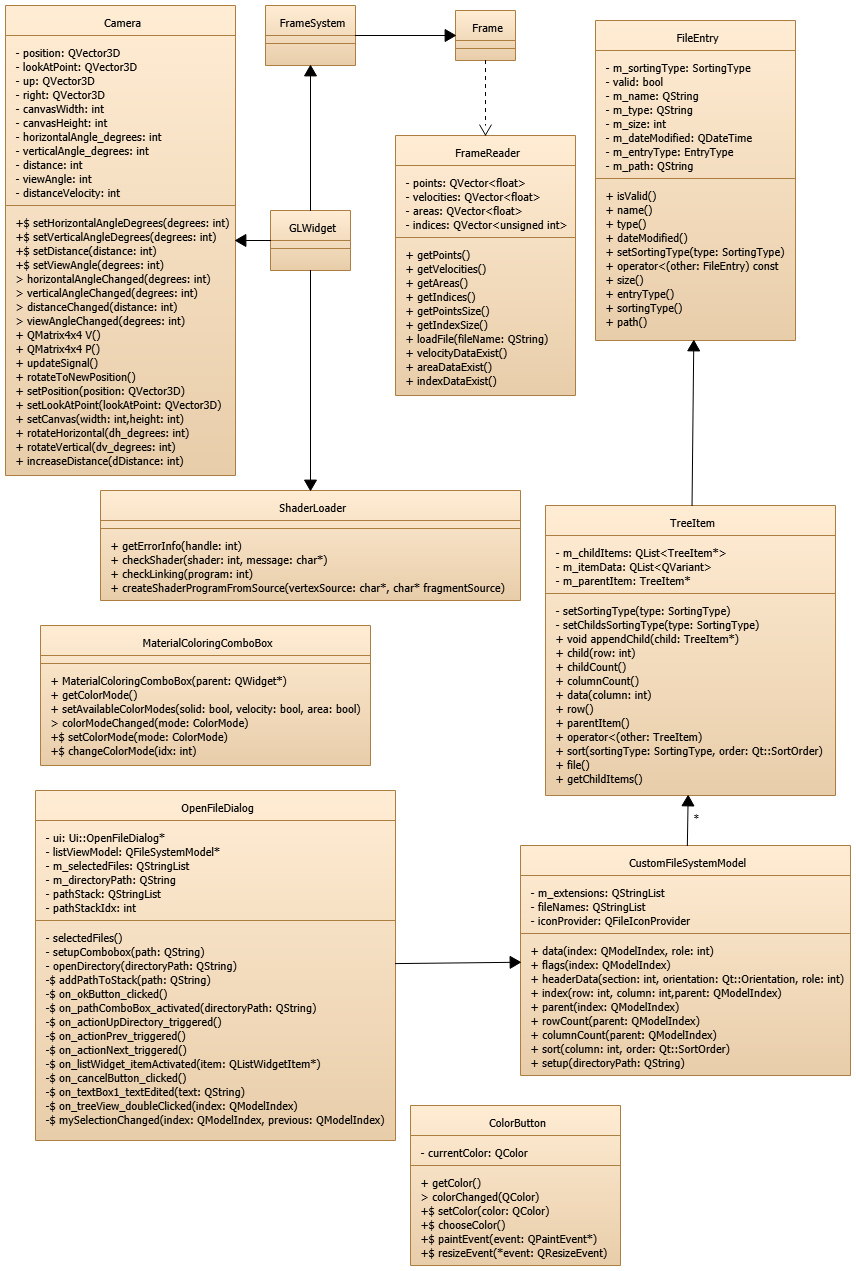
\includegraphics[scale=0.5]{thesis_class}
\caption{A vtp megjelenítő alkalmazás osztálydiagramja}
\label{fig:x thesis_class}
\end{figure}

\begin{description}[font=\normalfont\itshape\space]
\item [Camera:]
Feladata a kamera paramétereinek tárolása, 
a kamera mozgatása, valamint 
a megjelenítési tér középpontja körül történő forgatás. 
Tartalmaz signal -okat és slot -okat, 
amik segítségével egyrészt értesíti 
a felhasználói felületet állapotának megváltozásáról, 
másrészt lehetővé teszi a kamera paramétereinek hozzákötését 
a felhasználói felület elemeihez.
\item [ColorButton:]
A színkiválasztó gombot valósítja meg.
\item [CustomFileSystemModel:]
Egy olyan FileSystemModel, 
amiben az azonos nevű számozott fájlok fájlcsoportokat alkotnak. 
A fájlkiválasztó ablak használja.
\item [FileEntry:]
A {\ttfamily CustomFileSystemModel} -ben ez az osztály tartalmazza 
a fájlokkal kapcsolatban az olyan értékeket, 
mint például a fájl neve, típusa és mérete. 
Ide kerültek a fájlok rendezési szabályai is.
\item [Frame:]
Egy betöltött vtp fájlnak felel meg. 
Itt történik a betöltött adatok tárolása, 
valamint az egyes pontok (vagy vertexek) színeinek meghatározása.
\item [FrameReader:]
Az osztály feladata a vtp fájlok betöltése egy megadott elérési út alapján.
\item [FrameSystem:]
Az osztály feladata, 
hogy betöltse a frame -eket egy elérési út lista alapján, 
valamint hogy biztosítsa az OpenGL számára 
a frame -ek kirajzolásához szükséges bemenetet. 
Az osztálynak fontos szerepe van az egyes pontok színeinek meghatározásában is, 
mivel a szín nem csak az adott fájl pontjain múlik, 
hanem az összes frame összes pontját számításba kell venni.
\item [GLWidget:]
Ez az osztály felel a grafikus felhasználói felület 
közepén lévő OpenGL ablak tartalmáért, 
valamint itt történik 
a dock -olható paneleken és a toolbar -okon található 
beállítások összekötése az alkalmazás logikájával.
\item [MainWindow:]
Egy {\ttfamily QMainWindow} leszármazott osztály, 
ami a grafikus felhasználói felület alapját képezi. 
Itt történik felhasználói felület inicializálásának egy része.
\item [MaterialColoringComboBox:]
Ez az osztály valósítja meg azt a {\ttfamily QComboBox} -ot, 
amin kiválasztható, 
melyik vtp fájlból betöltött érték szerint legyen meghatározva rendereléskor 
az egyes pontok színe.
\item [OpenFileDialog:]
Az alkalmazásban található fájlkiválasztó ablakot valósítja meg.
\item [OpenGLInterface:]
Az osztály célja, hogy az OpenGL függvényeket 
a {\ttfamily GLWidget} osztályon kívül is lehessen használni 
a {\ttfamily GLWidget} -re történő rajzoláshoz. 
Egyelőre csak a shaderek betöltéséhez 
szükséges függvényeket tartalmazza.
\item [ShaderLoader:]
Van benne egy statikus függvény, 
ami a paraméterként átadott GLSL nyelven írt vertex 
és fragment shader kódokat lefordítja és betölti az OpenGL -be, 
majd visszatér a shader program azonosítószámával.
\item [TreeItem:]
A {\ttfamily CustomFileSystemModel} -ben ez az osztály felel meg 
az egyes fájloknak és mappáknak.
Egy {\ttfamily FileEntry} -ben tartalmazza a tényleges információkat 
a fájllal/mappával kapcsolatban.
\end{description}

\noindent A fejezet további részében a vtp megjelenítő alkalmazás megvalósítási részleteiről lesz szó.

\subsection{ColorButton}

A színek kiválasztásához szükség volt egy olyan felületelemre, 
amire kattintva a szín egyszerűen kiválasztható, 
majd a kiválasztott szín magán a felületelemen is megjelenik. 
Az is jó lett volna, ha a felületelem képes a 
Qt signal/slot rendszerén keresztül értesíteni, 
valamint értesülni a szín változásáról. 
Sajnos a Qt felhasználói felülete alapból nem tartalmaz ilyen elemet, 
így írni kellett egyet. 
A probléma egy {\ttfamily QPushButton} leszármazott osztállyal lett megoldva, 
ami gombnyomásra feldob egy {\ttfamily QColorDialog} -ot. 
Ezt úgy valósítottam meg, 
hogy a leszármazott osztályba betettem 
egy {\ttfamily chooseColor} slot -ot, 
amit rákötöttem a gomb {\ttfamily clicked} signal -jára. 
Így ha a felhasználó a gombra kattint,
a {\ttfamily chooseColor} függvény hívódik meg,
ami feldobja a {\ttfamily QColorDialog} -ot.
Ennek eredménye aztán elmentődik 
az osztályban található {\ttfamily currentColor} változóba. 

Hogy látható legyen, 
milyen szín került kiválasztásra, 
a {\ttfamily ColorButton} -ra felületén mindig szerepel egy, 
a {\ttfamily currentColor} változóban megadott színű kitöltött téglalap is. 

A {\ttfamily ColorButton} a kommunikációhoz felhasználja a Qt signal/slot rendszerét. 
A szín megváltozásáról egy {\ttfamily QColor} paramétert tartalmazó signal értesít, 
a szín kívülről történő beállítása pedig egy slot -on keresztül történik.

\subsection{MaterialColoringCombobox}

A vtp fájlok pontjainak színezéséhez szükség volt egy olyan felületelemre, 
amin ki lehet választani, 
hogy a színezés simán egy megadott színnel, 
vagy a {\ttfamily „velocity”}, {\ttfamily „vertex mass”}, {\ttfamily „vertex area”} 
és {\ttfamily „projected vertex area”} attribútumok valamelyike szerint történjen. 
A problémát egy sima {\ttfamily QComboBox} is megoldhatta volna, 
azonban az is fontos volt, 
hogy a sima színezést leszámítva a többi lehetőség csak akkor jelenjen meg rajta, 
ha a szükséges értékeket a betöltött fájl tartalmazza.

Emiatt az alkalmazásba végül egy {\ttfamily MaterialColoringCombobox} nevű 
{\ttfamily QComboBox} leszármazott osztály került. 
\\
A {\ttfamily MaterialColoringCombobox} megvalósításának főbb jellemzői:
\begin{itemize}
\item
Az aktuálisan kiválasztott színezési módot egy {\ttfamily ColorMode} enum tárolja.
\item
A {\ttfamily MaterialColoringCombobox} -ot 
inicializálni a {\ttfamily setAvailableColorModes} függvénnyel lehet, 
ami a ComboBox -ba betölti 
a lehetséges opciókat {\ttfamily QString} -ek formájában.
\item
Az osztályban van egy {\ttfamily setColorMode} slot, 
ami az átadott paraméter alapján beállítja 
az osztály {\ttfamily colorMode} változóját, 
majd a {\ttfamily setCurrentIndex} hívással átállítja 
a {\ttfamily QComboBox} ősben az aktuálisan kiválasztott értéket.
\item
Található az osztályban egy {\ttfamily changeColorMode} slot 
és egy {\ttfamily colorModeChanged} signal is. 
A {\ttfamily changeColorMode} annyit csinál, 
hogy meghívja az átadott index alapján megállapított színezési móddal 
a {\ttfamily setColorMode} slot -ot, 
majd emittál egy {\ttfamily colorModeChanged} signal -t.
\end{itemize}

\subsection{Kamera}

A kamera osztály legfontosabb feladata a felhasználói felületen megadott értékek, 
illetve az ott történő események (Pl.: egér mozgatás) alapján 
a kamera aktuális helyzetének megállapítása és tárolása, 
valamint az OpenGL által használt Projection és View mátrixok kiszámítása.

A kamera aktuális állapotát három változó tárolja: 
a pozíció és nézőpont vektorok, valamint a látószög. 
A Projection és View mátrixok kiszámítása ezen változók alapján történik. 
 
A kamerában van további három egész típusú változó is, 
amik a vízszintes és függőleges szöget, 
valamint a középponttól való távolságot tárolják. 
Ezeknek a képalkotás szempontjából közvetlenül nincsen szerepük, 
az osztályba csak a Qt grafikus felhasználói felületével 
való signal/slot alapú kommunikáció miatt kerültek. 
Ennek megfelelően a három változóhoz az osztályba természetesen került 
egy azok megváltozásáról értesítő signal, 
továbbá a változók értéke beállítható slot -ok segítségével. 
A változók tárolására egészek helyett célszerűbb 
lett volna lebegőpontos értékeket használni, 
azonban a Qt -ban nincs lebegőpontos slider, ami megnehezítette volna az változók szinkronizálását. 

A kamera pozíciójának meghatározása a vízszintes és függőleges szögek, 
valamint a {\ttfamily distance} változó alapján a következő algoritmussal történik:
\begin{enumerate}
\item
A program kiindul egy z tengely irányába mutató, 
a {\ttfamily distance} változónak megfelelő hosszúságú vektorból. 
Ez lesz a pozícióvektor. 
Felvesz egy {\ttfamily right} vektort is, 
aminek kezdeti értéke egy x tengely irányába mutató egységvektor. 
\item
A két vektort elforgatja az y tengely körül a vízszintes szöggel.
\item
A pozícióvektort elforgatja az elforgatott {\ttfamily right} vektor körül 
a függőleges szöggel.
\end{enumerate}

\subsection{A vtp fájlok betöltése}

A vtp fájlok betöltése a következő séma szerint történik:
\begin{enumerate}
\item
A felhasználó megnyomja az Open File gombot a felhasználói felületen. 
Ennek hatására meghívódik a {\ttfamily MainWindow} megfelelő eseménykezelő eljárása.
\item
Az eljárás feldob egy fájlkiválasztó ablakot, 
ami a felhasználóval való interakció után visszatér a betöltendő fájlok listájával.
\item
A {\ttfamily MainWindow} a {\ttfamily GLWidget} -en keresztül közvetetten 
meghívja a {\ttfamily FrameSystem} {\ttfamily loadFiles} függvényét, 
ami végigmegy az egyes fájlneveken és átadja őket 
a {\ttfamily Frame} osztály konstruktorának. 
A programban minden betöltött vtp fájlt egy {\ttfamily Frame} objektum reprezentál.
\item
A {\ttfamily Frame} konstruktora az átadott fájlnév alapján meghívja 
a {\ttfamily FrameReader} osztály {\ttfamily loadFile} függvényét, 
ami betölti a vtp fájl tartalmát.
\item
A {\ttfamily Frame} lekérdezi 
a fájlokban található adatokat a {\ttfamily FrameReader} -től, 
majd az adatok alapján feltölti belső változóit.
\item
A {\ttfamily FrameSystem} a vtp fájlok betöltése után végigmegy 
a {\ttfamily Frame} -eken 
és beállítja a {\ttfamily Frame} -ekben szereplő pontok/vertex -ek színeit.
\end{enumerate}

\subsection{FrameReader}

A {\ttfamily FrameReader} legfontosabb függvénye a {\ttfamily loadFile}, 
aminek feladata, 
hogy az átadott elérési úton található fájlból 
egy {\ttfamily QXmlStreamReader} segítségével betöltse a vertex vagy részecskepozíció, 
a sebesség, az area, valamint az index értékeket, 
amiket aztán a eltárol a {\ttfamily points}, 
a {\ttfamily velocities}, 
az {\ttfamily areas} és az {\ttfamily indices} tömbökben.

A tömbök tartalma a {\ttfamily loadFile} hívása után 
getter függvényekkel kérdezhető le. 
Mivel ezek visszatérési értéke nem pointer, 
bekerült az osztálya egy {\ttfamily velocityDataExist}, {\ttfamily indexDataExist} 
és {\ttfamily areaDataExist} függvény is. \\
Az egyes tömbök betöltésének menete a {\ttfamily loadFile} -ban:
\begin{enumerate}
\item
A program ellenőrzi, hogy az átadott elérési úton létezik -e a fájl.
\item
Ha létezik, egy {\ttfamily QXmlStreamReader} segítségével 
egy while ciklusban végigmegy rajta 
és a megtalált adatokat szövegként kiolvassa, 
majd négy darab stringbe tölti ({\ttfamily point}, {\ttfamily velocity}, 
{\ttfamily area}, {\ttfamily index}).
\item
A betöltött stringeket feldarabolja space -ek szerint. 
Az egyes darabokban ekkor a számok lesznek szöveg formátumban.
\item
A lista elemeit egyenként átkonvertálja lebegőpontos, 
vagy indexek esetén egész típusú változókká.
\end{enumerate}

\subsection{A pontok színeinek meghatározása}

Az egyes pontok/vertexek színeinek meghatározása 
a {\ttfamily Frame} és {\ttfamily FrameSystem} osztályok feladata. 
Solid módban a színezés egyszerű, 
hiszen az alkalmazásnak csak végig kell menni a {\ttfamily Frame} -eken 
és mindegyiknél meg kell hívnia a színbeállító függvényt.

A {\ttfamily velocity}, {\ttfamily vertex area}, 
{\ttfamily vertex mass} és {\ttfamily projected vertex area} szerint történő színezés 
az alább részletezett algoritmus szerint történik:
\begin{enumerate}
\item
A program végigmegy a {\ttfamily Frame} -eken és lekérdezi belőlük 
a színezési módnak megfelelő tömb -ből a legkisebb, 
valamint a legnagyobb értéket. 
Ez {\ttfamily vertex area}, {\ttfamily vertex mass} és 
{\ttfamily projected vertex area} esetén egy sima minimum, 
illetve maximumkeresést jelent, 
míg {\ttfamily velocity} esetén a keresés a vektor abszolút értéke szerint történik.
\item
A program végigmegy a legkisebb és legnagyobb értékeken 
és ezeken is végrehajt egy minimum, illetve maximum keresést. 
Végül megtalálja az összes {\ttfamily Frame} -re együttesen jellemző 
legkisebb és legnagyobb értéket.
\item
A minden {\ttfamily Frame} -nek átadja a felhasználói felületen beállítható 
start és end color színeket, 
valamint a minimális és maximális értékeket.
\item
Az egyes {\ttfamily Frame} -ek ezután végigmennek a bennük található összes háromszögponton 
és lineáris interpolációval beállítják a színt attól függően, 
hogy a ponthoz tartozó érték a minimum vagy maximumértékhez van -e közelebb.
\end{enumerate}

\subsection{A Frame kirajzolása}

A program a kirajzolásra két lehetőséget kínál fel, 
amik a pont és háromszögrajzoló mód. 
Ennek oka, hogy a betöltendő fájlok között van olyan, 
ami nem tartalmaz információt arról, 
hogy a pontokat milyen sorrendben kell az OpenGL -nek megadni, 
viszont a fájlban szereplő sorrend
háromszögek kirajzolására biztosan nem alkalmas. 
Ilyenkor az alkalmazás alapértelmezetten
pontokat rajzol háromszögek helyett.

Az alkalmazás a háromszögrajzoló módhoz az OpenGL indexelés funkcióját használja. 
Ennek lényege, hogy az OpenGL -ben 
a háromszögpontok megadása nem a pontok pozícióit tartalmazó bufferrel történik, 
hanem egy indexbuffer segítségével, 
amiben az egyes értékek azt jelzik, 
hogy az adott háromszögpont pozíciója a vertexbuffer hanyadik eleme. 
Az indexelés egyébként pont megfelel a vtp fájlokban található adatok betöltésére, 
mivel ott az indexek úgy lettek meghatározva, 
hogy változtatás nélkül átadhatóak legyenek az OpenGL -nek. 
Ennek megfelelően az animáció kirajzolása egyszerűen úgy történik, 
hogy a {\ttfamily GLWidget} lekérdezi 
a {\ttfamily FrameSystem} -ből a tömböket, 
amik a vertex -eket, színeket és indexeket tárolják, 
majd egyszerűen betölti azokat az OpenGL buffereibe. 
Ezután következik a fényforrással kapcsolatos paraméterek, 
valamint a kamera V és P mátrixának megadása, 
majd az OpenGL {\ttfamily „drawElements”} függvényének meghívása.

\subsection{Megvilágítás}

A megvilágítás a prt megjelenítő alkalmazással ellentétben 
a Phong árnyalási modellt használja. 
Ehhez a shader -ek egy darab pontfényforrást használnak. \\
A megvilágítással kapcsolatban a {\ttfamily GLWidget} osztály 
a következő paramétereket tartja nyilván:
\begin{description}[font=\normalfont\itshape\space]
\item [lightPosition:]
A fényforrás pozíciója világ koordináta -rendszerben. 
\item [lightPower:]
Egy szám, 
amivel a kiszámolt diffúz és spekuláris szín megszorzódik a shaderben.
\item [specularPower:]
A szám 0 és 100 közötti értéket vehet fel. 
A program a számot az OpenGL -nek való átadása előtt átkonvertálja lebegőpontos értékre 
és elosztja 100 -zal. 
Így egy 0 és 1 közötti szám keletkezik, 
amivel a fragment shader beszorozza a kiszámolt spekuláris színt.
\item [smoothness:]
A felület simaságának mértéke. 
Az érték átalakítás nélkül kerül az OpenGL megjelenítési csővezetékébe, 
ahol a shader a spekuláris szín kiszámításához használja.
\item [ambientPower:]
A specularPower -hez hasonlóan szintén csak 0 és 100 közötti értéket vehet fel, 
amit a program átalakít egy 0 és 1 közötti lebegőpontos értékre. 
Az így kapott szám megszorzódik a shaderben az ambiens színnel.
\end{description}

A {\ttfamily GLWidget} -ben a pozíciót leszámítva 
a fénnyel kapcsolatos paraméterek egész értékűek. 
Ennek oka, hogy a felhasználói felületen 
a paraméterek beállítását segítő {\ttfamily QSlider} -ekkel 
csak egész értékeket lehet kezelni, lebegőpontosokat nem. 
A problémát egyébként meg lehetett volna oldani 
egy lebegőpontos értéket támogató {\ttfamily QSlider} implementálásával is, 
azonban egyszerűbb egészekkel számolni, 
amik csak az OpenGL -lel való interakció folyamán konvertálódnak át.

A Phong árnyalási modell implementálásához szükség van a felület normálvektoraira is. 
Sajnos azonban a betöltendő vtp fájlokból a normálvektorok hiányoznak, 
amik kiszámítása így a programra hárul. 
A normálvektorok kiszámítása a fragment shader -ben történik 
az OpenGL beépített {\ttfamily dFdx} és {\ttfamily dFdy} függvényével. 
Az eljárás lényege, hogy a vertex shader -ben kiszámolásra kerül 
a vertex pozíciója kamera -koordinátarendszerben, 
aminek a pontok közötti interpolált értéke aztán megjelenik 
a fragment shader bemenetén. 
Az interpolált értéket a fragment shader átadja 
az OpenGL {\ttfamily dFdx} és {\ttfamily dFdy} függvényeinek, 
amik kiszámolják az x és y tengely szerinti parciális deriváltat, 
majd azt rögtön irányvektorrá is alakítják. 
A két vektor vektoriális szorzatát véve így már megkapható a felület normálvektora \cite{normalvector}. 
\\
Az normálvektort kiszámító kódsor:
\begin{lstlisting}[style=customcpp]
vec3 Normal_cameraspace = normalize(cross(dFdx(Position_cameraspace), dFdy(Position_cameraspace)));
\end{lstlisting}

\section{A fájlkiválasztó ablak}

A prt megjelenítő alkalmazás 
egyik legnagyobb hiányossága egy olyan felület, 
amin lehetőség van a betöltendő fájlok kiválasztására. 
A Qt ezt a problémát egy saját osztállyal oldja meg, 
ami megjeleníti az adott operációs rendszer 
beépített fájlkiválasztó ablakát. 
Sajnos a Windows megoldása azonban a célra nem felelt meg.
Az egyik probléma az volt,
hogy bár lehetőség van egyszerre több fájl kiválasztására, 
azt már nem lehetett megoldani, 
hogy az ablak csak olyan fájlokat engedjen egyszerre kiválasztani, 
amik ugyanahhoz az animációhoz tartoznak.
A másik hiányosság, hogy jó lett volna, 
ha az egy animációhoz tartozó fájlokat
a felületen lenyitható csoportokba lehet szervezni. 
A megoldás végül egy saját fájlkiválasztó ablak volt. 
Szerencsére a Qt Model/View widget -jeinek, a {\ttfamily QListView}
és {\ttfamily QTreeView} osztályoknak köszönhetően
ennek megvalósítása nem volt nehéz.

\subsection{A fájlkiválasztó ablak felhasználói felülete}

\begin{figure}[!htb]
\centering
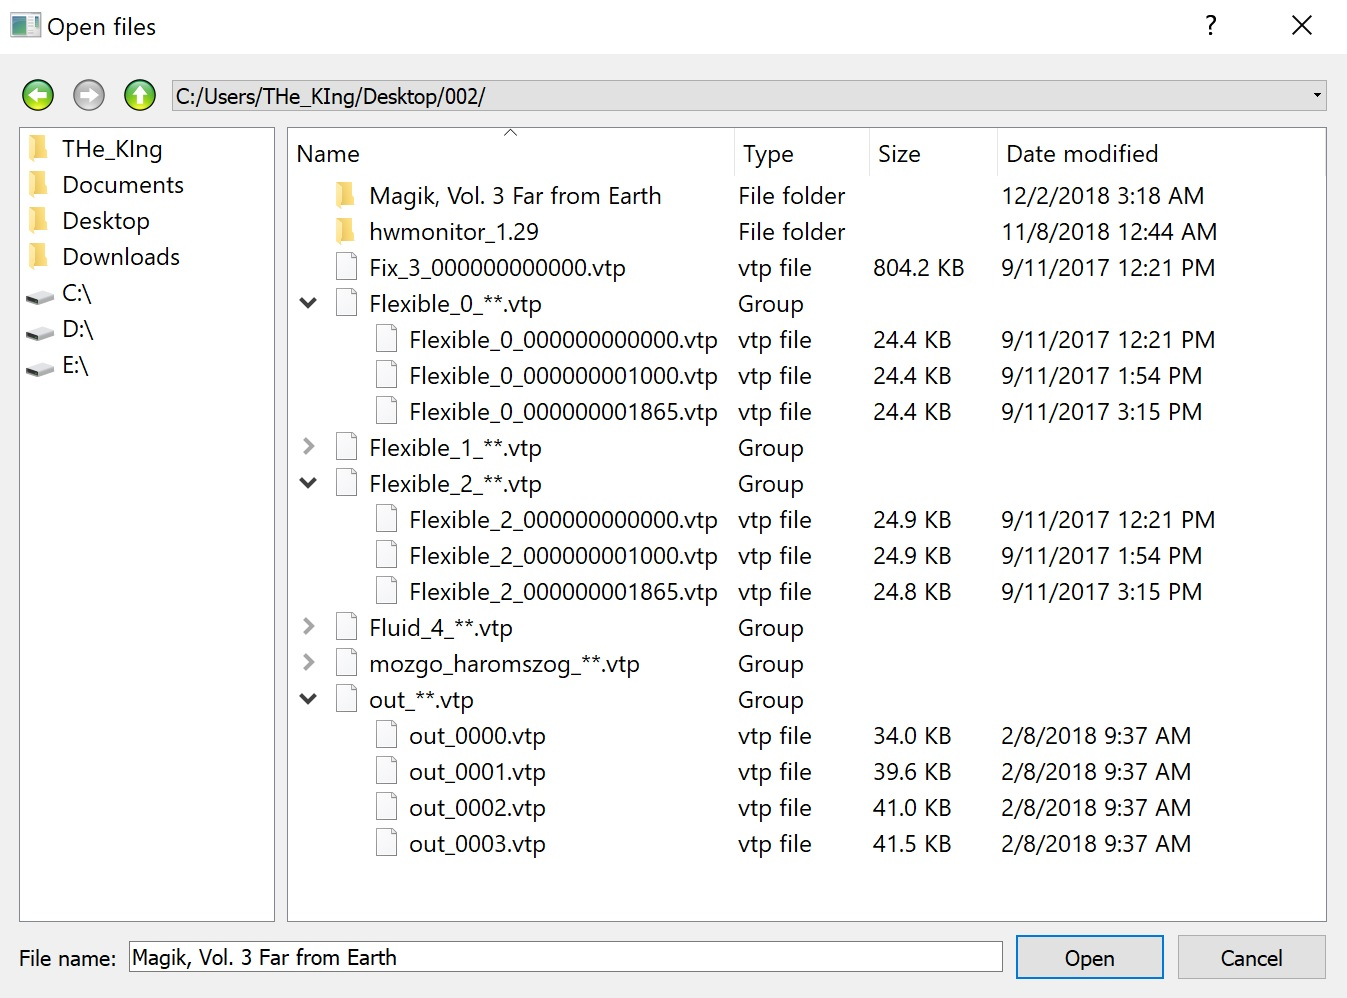
\includegraphics[scale=0.8]{openfiledialog}
\caption{A fájlkiválasztó ablak}
\label{fig:x openFileDialog}
\end{figure}

Ahogy a \ref{fig:x openFileDialog} ábrán is látható, 
a fájlkiválasztó készítésekor az volt a cél, 
hogy az ablak kinézetre a lehető legjobban hasonlítson 
a Windows operációs rendszeren megszokottra. 
Ennek megfelelően a felületen az elemek egy nagyobb 
és két kisebb sorban helyezkednek el.

Az első sorban három gomb és egy {\ttfamily QComboBox} található. 
A gombok funkciója ugyanaz, mint a Windows -os megfelelőiké. 
A vissza és tovább gombbal az eddig megnyitott mappák listáján lehet váltogatni, 
az up -al pedig a szülőkönyvtárba lehet ugrani. 
A {\ttfamily QComboBox} tartalma különbözik a Windows -ban megszokottól, 
mivel abban jellemzően megjelenik egy lista a korábban megnyitott mappákról, 
míg itt az egyes szülőkönyvtárak szerepelnek egészen a root -ig, 
vagy a meghajtó betűjeléig.

A második sorban két elem található. 
Az egyik egy listanézet, 
amin a fontosabb helyek jelennek meg. 
Ilyen a felhasználó nevével jelzett mappa a users -ben, 
a dokumentumok, a letöltések, valamint az asztal. 
Windows -on ezen kívül még megjelennek a meghajtók, 
míg Linuxon a root könyvtár is. 
A listanézet a mappák számát leszámítva 
kinézetre és funkció szempontjából megegyezik 
a Windows -ba beépített párbeszédablakon láthatóval. 
A másik elem egy {\ttfamily QTreeView}, 
amin az aktuális mappa tartalmának megjelenítése,
valamint a fájlok kiválasztása történik.
A {\ttfamily QTreeView} annyiban különbözik a Windows -os változattól, 
hogy egyszerre csak egy fájl kiválasztását engedi, 
viszont az azonos nevű számozott fájlokat
(tehát amik ugyanahhoz az animációhoz tartoznak)
lenyitható csoportokba szervezi, 
amiket így egyszerre is meg lehet nyitni.

Az utolsó sorban található egy szövegdoboz,
amin lehetőség van beírni a kiválasztandó fájl/csoport nevét. 
Ezenkívül természetesen ott van a szokásos Open és Cancel gomb is.

\subsection{A fájlkiválasztó ablak implementálása}

A fájlkiválasztó ablakon a Widget -ek adatokkal való feltöltése, 
valamint az eseménykezelő eljárások megírása alapvetően egyszerű volt, 
mivel a Qt ugyanazokat a mintákat követi, 
amiket a többi grafikus felhasználói felület is.

A legnagyobb problémát a középen látható
{\ttfamily QTreeView} feltöltése jelentette, 
ami a Qt Model/View programing elve alapján működik. 
Ez alapvetően nem lenne probléma, 
ha a célra megfelelne a Qt beépített {\ttfamily QFileSystemModel} osztálya is. 
A saját fájlkiválasztó ablakra viszont pont ennek
hiányosságai miatt volt szükség,
így a {\ttfamily QTreeView} -hez írni kellett 
egy saját Model osztályt, 
ami a {\ttfamily CustomFileSystemModel} nevet kapta.

A {\ttfamily CustomFileSystemModel} -hez ősosztálynak 
a {\ttfamily QAbstractItemModel} -re esett a választás. 
Lehetett volna a {\ttfamily QAbstractListModel} is, 
azonban a lenyitható fájlcsoportok miatt mindenképp fa struktúrára volt szükség, 
amit csak a {\ttfamily QAbstractItemModel} tud biztosítani. 
A választásban persze a Qt „simple tree example” példaprojektje 
is szerepet játszott, 
ami egyébként a kód alapját képezi.

\vspace{3mm}

\noindent{\itshape\bfseries A megjelenítendő adatok tárolása:}

\vspace{3mm}

A megjelenítendő adatok, azaz a mappák, 
fájlok és fájlcsoportok egy egyszerű fa struktúrában tárolódnak 
a {\ttfamily CustomFileSystemModel} osztályon belül. 
A fa három szintű. Az első szinten helyezkedik el a gyökérelem, 
amiben a {\ttfamily QTreeView} header -feliratai tárolódnak. 
A második szinten helyezkednek el azok a fájlok,
mappák, vagy csoportok, 
amik a felületen a fájlcsoportok lenyitása nélkül láthatóak. 
A fa legalsó szintjén azok a fájlok tárolódnak, 
amik valamely fájlcsoport tagjai.
\newline
A fa csomópontjait a {\ttfamily TreeItem} osztály valósítja meg. 
Egy {\ttfamily TreeItem} -nek 4 belső változója van: 
\begin{description}[font=\normalfont\itshape\space]
\item [sortingType:]
Ez határozza meg, hogy a {\ttfamily TreeItem} -ek 
rendezése melyik paraméter szerint történjen.
\item [childItems:]
Egy lista, amiben a csomópont gyerekelemeire mutató pointer -ek tárolódnak.
\item [itemData:]
Egy lista, ami a {\ttfamily QTreeView} -n megjelenítendő szövegeket 
tartalmazza {\ttfamily QString} -ként,
az oszlopok szerinti sorrendben.
\item [parentItem:]
Egy pointer a szülőcsomópontra.
\item [file:]
Egy {\ttfamily FileEntry} objektum, 
ami ugyanazokat az adatokat tartalmazza, 
mint az itemData, 
csak {\ttfamily QString} helyett mindegyiket a megfelelő típusban. 
A {\ttfamily file} objektum szerepe, 
hogy egyrészt biztosítja a Model indexek számára a fájlok adatainak kinyerhetőségét, 
másrészt rendezéskor itt történik a fájlok tényleges összehasonlítása 
egy {\ttfamily operator<} függvény segítségével. 
A működés folyamán gyakran szükség van a fa struktúra felszabadítására és újrainicializálására. 
Ennek oka, hogy csak a felületen is látható elemek tárolódnak, 
a fájlrendszer többi része nem. 
A fa felszabadítása rekurzívan történik, 
így {\ttfamily CustomFileSystemModel} -ben
csak egy darab felszabadító utasítás van,
ami a gyökérelemet szabadítja fel.
\end{description} 

\vspace{2mm}

\noindent{\itshape\bfseries A CustomFileSystemModel implementációja:}

\vspace{3mm}

\begin{sloppypar}
Az {\ttfamily CustomFileSystemModel} osztályt megpróbáltam úgy implementálni,  
hogy a Qt irányelveinek megfelelően 
a {\ttfamily QAbstractItemModel} meglévő függvényei 
csak minimálisan legyenek kibővítve. 
Ennek megfelelően az osztály csak egy darab ősosztályban 
nem szereplő publikus függvényt tartalmaz (a {\ttfamily setup} függvény), 
ami az aktuális mappa megadására jó. 
\\
Az osztály használata a következő pontokban foglalható össze: 
\end{sloppypar}

\begin{itemize}
\item
Először meg kell hívni a konstruktort, 
amiben át kell adni a megjelenítendő fájlok kiterjesztéseit egy listában. 
Ez egyelőre csak vtp fájlokkal működik.
\item
A {\ttfamily QTreeView} -nek történő átadás előtt 
meg kell hívni a {\ttfamily setup} függvényt, 
amiben át kell adni a megjelenítendő könyvtár elérési útját.
\item
Ha kattintás történik valamin, 
a kapott indexből lekérdezhető egy pointer 
a mögöttes {\ttfamily TreeItem} -re, 
amiből aztán minden információ kinyerhető.
\item
A Model mindig csak az aktuálisan megnyitott mappa tartalmát tárolja. 
A mappát szükség esetén kívülről lehet megváltoztatni
egy {\ttfamily setup} hívással.
\end{itemize}

\begin{sloppypar}
A {\ttfamily CustomFileSystemModel} működéséhez felül kellett 
definiálni párat a {\ttfamily QAbstractItemModel} függvényei közül. 
A következőkben ezen függvények implementációs részletei kerülnek bemutatásra:

\begin{description}[font=\normalfont\itshape\space]
\item [data:]
{\ttfamily Qt::DisplayRole} szerep esetén a {\ttfamily TreeItem} -től 
közvetlenül lekérdezhető a megjelenítendő adatok listája,
{\ttfamily Qt::DecorationRole} -nál pedig
a függvénynek vissza kell térnie egy ikonnal, 
amihez először a 
{\ttfamily TreeItem} -ben található {\ttfamily FileEntry} objektum alapján eldönti, 
hogy az adat fájlra, vagy mappára vonatkozik -e, 
majd a megfelelő ikont a {\ttfamily QFileIconProvider} osztálytól szerzi meg. 
\item [headerData:]
A függvény feladata, hogy visszatérjen 
az oszlopok tetején látható 
header szövegekkel (Például: "Name","Type","Size"). 
Ezek a gyökérelem
{\ttfamily m\_itemData} változójában találhatóak.
\item [index:]
A függvény először a parent index alapján szerez egy pointert 
a szülő {\ttfamily TreeItem} -re. 
Konvenció alapján ha a szülőindex érvénytelen, 
az a gyökérelemet jelenti. 
Ezután visszatér a sornak és oszlopnak megfelelő gyerekelem indexével, 
amire a szabály, 
hogy a fa struktúrában minden sorhoz egy darab {\ttfamily TreeItem} tartozik 
és ennek a gyerekek listájában elfoglalt helye megegyezik 
a sor számával (Tehát egy soron belül 
az {\ttfamily internalPointer} függvény minden elemnél ugyanarra 
a {\ttfamily TreeItem} objektumra fog mutatni).
\item [parent:]
A függvénynek az átadott index alapján
vissza kell térnie a szülőelem indexével. 
Szerencsére egy {\ttfamily TreeItem} mindig tartalmaz pointer -t a szülőelemre, 
így ez könnyen elkészíthető.
\item [rowCount:]
A sorok száma természetesen a gyerekek számával egyezik meg. 
\item [columnCount:]
Az oszlopok száma azonos a megjelenítendő adatok listájának elemszámával.
\item [sort:]
A függvény két paramétert vesz át. 
Az egyik a rendezés alapjául szolgáló oszlop száma, 
a másik a rendezés iránya,
ami lehet növekvő, vagy csökkenő. 
A függvény az oszlopszám alapján először kiolvassa a gyökérelemből 
az oszlophoz tartozó header feliratot. 
Ezután egy {\ttfamily QMap} -hez fordul, 
ami az egyes header feliratokhoz rendel {\ttfamily sortingType} enum -okat. 
Az így kiolvasott {\ttfamily sortingType} lesz a rendezési típus, 
amit már át tud adni a rendezés irányával együtt 
a {\ttfamily rootItem} {\ttfamily sort} függvényének.
\end{description}
\end{sloppypar}

Ahogy a fenti leírásból is látszik, 
a {\ttfamily QAbstractItemModel} függvényeit nem volt nehéz implementálni, 
mivel egy kész fa struktúrát kaptak. 
Ennek a felépítése a {\ttfamily setup} függvényben történik 
a következő lépések szerint:
\begin{description}[font=\normalfont
\stepcounter{descriptcount}\arabic{descriptcount}.~]
\item [\textit{A meglévő gyökérelem törlése:}]
Az új tartalom megjelenítéséhez először törölni kell a meglévőt.
Mivel minden csomópont maga felel 
a gyerekcsomópontok felszabadításáért, 
a gyökérelem felszabadítása elegendő.
\item [\textit{Az új gyökérelem elkészítése:}]
Ebbe egy üres {\ttfamily FileEntry} kerül, 
valamint a {\ttfamily data} függvény számára 
az oszlopok header feliratai.
\item [{\itshape A mappákhoz tartozó csomópontok hozzáadása:}]
A függvény először a {\ttfamily QDir} osztálytól lekérdez 
egy listát a mappákról, 
majd minden mappa alapján csinál 
egy azt reprezentáló {\ttfamily TreeItem} -et, 
amit hozzáad a gyökérelem gyerekcsomópont listájához.
\item [\textit{Fájlcsoportok keresése:}]
Ehhez a függvény először egy {\ttfamily QMap} -et csinál, 
ami {\ttfamily QString} kulcsokhoz rendel {\ttfamily FileEntry} listákat. 
Ezután végigmegy a fájlokon és 
egy reguláris kifejezés segítségével mindegyiknél ellenőrzi, 
hogy a neve számozott -e. 
Amennyiben számozott fájlról van szó, 
a fájlnév alapján megállapít egy csoportnevet. 
Ez a csoportnév lesz a kulcs a {\ttfamily QMap} -ben ahhoz a listához, 
amelyikbe a fájl kerül. 
Amennyiben a fájl nem számozott, 
a kulcs a csoportnév helyett simán a fájlnév lesz. 
A folyamat végére keletkezik egy {\ttfamily QMap}, 
amiben a kulcsok a csoportnevek, 
az értékek pedig a csoportokhoz tartozó fájlok lesznek. 
\item [\textit{A fájlok és fájlcsoportok hozzáadása:}]
A függvény végigiterál a {\ttfamily QMap} -ben található csoportokon. 
Ha a csoportban csak egy fájl van, 
a fájlról egyszerűen csinál egy {\ttfamily TreeItem} -et, 
amit hozzáad a gyökérelem gyerekcsomópontjaihoz. 
Ha több fájl is található, 
a függvény először egy fájlcsoport típusú {\ttfamily TreeItem} -et csinál, 
ami a {\ttfamily QMap} kulcsot kapja névként. 
A csoportban található fájlok ennek a gyerekei lesznek. 
\end{description}

\vspace{2mm}

\noindent{\itshape\bfseries A QTreeView rendezése:}

\vspace{3mm}

A {\ttfamily QTreeView} tartalma természetesen rendezhető név, típus, méret 
és módosítási dátum alapján. 
Mivel a megjelenített fájlok és mappák sorrendje megegyezik 
a gyökérelem gyerekcsomópontjainak sorrendjével, 
a rendezés a {\ttfamily TreeItem} -ben történik. 
\newline
A rendezést végző algoritmus jellemzői:
\begin{itemize}
\item
Fontos volt, hogy mappák mindig a fájlok és fájlcsoportok előtt legyenek. 
Ennek eléréshez az algoritmus először különválasztja két listába 
a mappákat és a fájlokat, majd külön rendezi őket. 
A gyerekcsomópontok új listája a két rendezett lista összefűzésével keletkezik. 
\item
A mappák nem tartalmaznak információt a méretről, 
így méret szerinti rendezés esetén is név szerint rendeződnek. 
\item
Mivel rendezéskor a mappák külön listában vannak, 
a típusuk nem különbözik egymástól, 
így a mappáknál típus esetén is név szerinti rendezés van beállítva.
\item
Fájlcsoportok esetén a rendezőlistához való hozzáadás előtt 
a csoportok tartalmát is rendezni kell, 
ami egy rekurzív {\ttfamily sort} hívással történik.
\item
Mivel a gyerekelemek listájában pointerek vannak, 
a Qt rendező függvényéhez csinálni kellett két összehasonlító függvényt is. 
Az egyik növekvő, a másik csökkenő sorrendhez kell. 
A {\ttfamily TreeItem} {\ttfamily sort}
függvényében a függvény végén 
található switch -re azért volt szükség, 
mert név és típus alapján történő rendezés esetén 
a mappáknak mindig név szerint növekvő sorrendben kell lenniük,
még akkor is, ha a rendezés egyébként csökkenő sorrendben történik.
\end{itemize}
